% Options for packages loaded elsewhere
\PassOptionsToPackage{unicode}{hyperref}
\PassOptionsToPackage{hyphens}{url}
%
\documentclass[
]{book}
\usepackage{amsmath,amssymb}
\usepackage{lmodern}
\usepackage{iftex}
\ifPDFTeX
  \usepackage[T1]{fontenc}
  \usepackage[utf8]{inputenc}
  \usepackage{textcomp} % provide euro and other symbols
\else % if luatex or xetex
  \usepackage{unicode-math}
  \defaultfontfeatures{Scale=MatchLowercase}
  \defaultfontfeatures[\rmfamily]{Ligatures=TeX,Scale=1}
\fi
% Use upquote if available, for straight quotes in verbatim environments
\IfFileExists{upquote.sty}{\usepackage{upquote}}{}
\IfFileExists{microtype.sty}{% use microtype if available
  \usepackage[]{microtype}
  \UseMicrotypeSet[protrusion]{basicmath} % disable protrusion for tt fonts
}{}
\makeatletter
\@ifundefined{KOMAClassName}{% if non-KOMA class
  \IfFileExists{parskip.sty}{%
    \usepackage{parskip}
  }{% else
    \setlength{\parindent}{0pt}
    \setlength{\parskip}{6pt plus 2pt minus 1pt}}
}{% if KOMA class
  \KOMAoptions{parskip=half}}
\makeatother
\usepackage{xcolor}
\IfFileExists{xurl.sty}{\usepackage{xurl}}{} % add URL line breaks if available
\IfFileExists{bookmark.sty}{\usepackage{bookmark}}{\usepackage{hyperref}}
\hypersetup{
  pdftitle={Digital Skills},
  hidelinks,
  pdfcreator={LaTeX via pandoc}}
\urlstyle{same} % disable monospaced font for URLs
\usepackage{color}
\usepackage{fancyvrb}
\newcommand{\VerbBar}{|}
\newcommand{\VERB}{\Verb[commandchars=\\\{\}]}
\DefineVerbatimEnvironment{Highlighting}{Verbatim}{commandchars=\\\{\}}
% Add ',fontsize=\small' for more characters per line
\usepackage{framed}
\definecolor{shadecolor}{RGB}{248,248,248}
\newenvironment{Shaded}{\begin{snugshade}}{\end{snugshade}}
\newcommand{\AlertTok}[1]{\textcolor[rgb]{0.94,0.16,0.16}{#1}}
\newcommand{\AnnotationTok}[1]{\textcolor[rgb]{0.56,0.35,0.01}{\textbf{\textit{#1}}}}
\newcommand{\AttributeTok}[1]{\textcolor[rgb]{0.77,0.63,0.00}{#1}}
\newcommand{\BaseNTok}[1]{\textcolor[rgb]{0.00,0.00,0.81}{#1}}
\newcommand{\BuiltInTok}[1]{#1}
\newcommand{\CharTok}[1]{\textcolor[rgb]{0.31,0.60,0.02}{#1}}
\newcommand{\CommentTok}[1]{\textcolor[rgb]{0.56,0.35,0.01}{\textit{#1}}}
\newcommand{\CommentVarTok}[1]{\textcolor[rgb]{0.56,0.35,0.01}{\textbf{\textit{#1}}}}
\newcommand{\ConstantTok}[1]{\textcolor[rgb]{0.00,0.00,0.00}{#1}}
\newcommand{\ControlFlowTok}[1]{\textcolor[rgb]{0.13,0.29,0.53}{\textbf{#1}}}
\newcommand{\DataTypeTok}[1]{\textcolor[rgb]{0.13,0.29,0.53}{#1}}
\newcommand{\DecValTok}[1]{\textcolor[rgb]{0.00,0.00,0.81}{#1}}
\newcommand{\DocumentationTok}[1]{\textcolor[rgb]{0.56,0.35,0.01}{\textbf{\textit{#1}}}}
\newcommand{\ErrorTok}[1]{\textcolor[rgb]{0.64,0.00,0.00}{\textbf{#1}}}
\newcommand{\ExtensionTok}[1]{#1}
\newcommand{\FloatTok}[1]{\textcolor[rgb]{0.00,0.00,0.81}{#1}}
\newcommand{\FunctionTok}[1]{\textcolor[rgb]{0.00,0.00,0.00}{#1}}
\newcommand{\ImportTok}[1]{#1}
\newcommand{\InformationTok}[1]{\textcolor[rgb]{0.56,0.35,0.01}{\textbf{\textit{#1}}}}
\newcommand{\KeywordTok}[1]{\textcolor[rgb]{0.13,0.29,0.53}{\textbf{#1}}}
\newcommand{\NormalTok}[1]{#1}
\newcommand{\OperatorTok}[1]{\textcolor[rgb]{0.81,0.36,0.00}{\textbf{#1}}}
\newcommand{\OtherTok}[1]{\textcolor[rgb]{0.56,0.35,0.01}{#1}}
\newcommand{\PreprocessorTok}[1]{\textcolor[rgb]{0.56,0.35,0.01}{\textit{#1}}}
\newcommand{\RegionMarkerTok}[1]{#1}
\newcommand{\SpecialCharTok}[1]{\textcolor[rgb]{0.00,0.00,0.00}{#1}}
\newcommand{\SpecialStringTok}[1]{\textcolor[rgb]{0.31,0.60,0.02}{#1}}
\newcommand{\StringTok}[1]{\textcolor[rgb]{0.31,0.60,0.02}{#1}}
\newcommand{\VariableTok}[1]{\textcolor[rgb]{0.00,0.00,0.00}{#1}}
\newcommand{\VerbatimStringTok}[1]{\textcolor[rgb]{0.31,0.60,0.02}{#1}}
\newcommand{\WarningTok}[1]{\textcolor[rgb]{0.56,0.35,0.01}{\textbf{\textit{#1}}}}
\usepackage{longtable,booktabs,array}
\usepackage{calc} % for calculating minipage widths
% Correct order of tables after \paragraph or \subparagraph
\usepackage{etoolbox}
\makeatletter
\patchcmd\longtable{\par}{\if@noskipsec\mbox{}\fi\par}{}{}
\makeatother
% Allow footnotes in longtable head/foot
\IfFileExists{footnotehyper.sty}{\usepackage{footnotehyper}}{\usepackage{footnote}}
\makesavenoteenv{longtable}
\usepackage{graphicx}
\makeatletter
\def\maxwidth{\ifdim\Gin@nat@width>\linewidth\linewidth\else\Gin@nat@width\fi}
\def\maxheight{\ifdim\Gin@nat@height>\textheight\textheight\else\Gin@nat@height\fi}
\makeatother
% Scale images if necessary, so that they will not overflow the page
% margins by default, and it is still possible to overwrite the defaults
% using explicit options in \includegraphics[width, height, ...]{}
\setkeys{Gin}{width=\maxwidth,height=\maxheight,keepaspectratio}
% Set default figure placement to htbp
\makeatletter
\def\fps@figure{htbp}
\makeatother
\setlength{\emergencystretch}{3em} % prevent overfull lines
\providecommand{\tightlist}{%
  \setlength{\itemsep}{0pt}\setlength{\parskip}{0pt}}
\setcounter{secnumdepth}{5}
\usepackage{booktabs}
\ifLuaTeX
  \usepackage{selnolig}  % disable illegal ligatures
\fi
\usepackage[]{natbib}
\bibliographystyle{apalike}

\title{Digital Skills}
\author{}
\date{\vspace{-2.5em}2022-07-03}

\begin{document}
\maketitle

{
\setcounter{tocdepth}{1}
\tableofcontents
}
\hypertarget{A-Note-About-this-Resource}{%
\chapter*{A Note About this Resource}\label{A-Note-About-this-Resource}}
\addcontentsline{toc}{chapter}{A Note About this Resource}

\begin{center}\rule{0.5\linewidth}{0.5pt}\end{center}

\textbf{What is this?}

This resource has been written using \textbf{R}, \textbf{LaTeX} and \textbf{R Studio} and published through \textbf{GitHub}. As the resource is hosted on GitHub it is available anywhere, any time and on any device. This resource supports the embedding of images, video content, html content (iframes), live code and mathematical formula and makes sharing the content much easier. In addition, this resource is capable of embedding Power BI dashboards, Python and R coded visuals.

\textbf{Contents}

\begin{itemize}
\tightlist
\item
  Statistics

  \begin{itemize}
  \tightlist
  \item
    Introduction
  \item
    Data Types and Levels of Measurement
  \item
    Describing Data
  \item
    Comparing Data
  \item
    Data Visualisation
  \end{itemize}
\item
  Power BI

  \begin{itemize}
  \tightlist
  \item
    Introduction
  \item
    Data Transformation
  \item
    Data Visualisation
  \end{itemize}
\item
  Python

  \begin{itemize}
  \tightlist
  \item
    Introduction
  \item
    Managing Data
  \item
    Data Visualisation
  \item
    Use Cases and Examples
  \end{itemize}
\item
  R

  \begin{itemize}
  \tightlist
  \item
    Introduction
  \item
    Managing Data
  \item
    Data Visualisation
  \item
    Use Cases and Examples
  \end{itemize}
\end{itemize}

\hypertarget{intro}{%
\chapter{Introduction}\label{intro}}

\begin{center}\rule{0.5\linewidth}{0.5pt}\end{center}

\hypertarget{what-is-statistics}{%
\section{What is Statistics?}\label{what-is-statistics}}

Statistics is all about the collection, organization, analysis, interpretation and presentation of data. Statistics is used everywhere from opinion polling in politics to predicting the prices of assets. There are two main branches of statistics: descriptive statistics and inferential statistics.

\hypertarget{descriptive-statistics}{%
\subsection{Descriptive Statistics}\label{descriptive-statistics}}

Descriptive statistics describes or summarises data that have been collected. Measures of central tendency such as (mean, median and the mode) and measures of dispersion (range, interquartile range and standard deviation) are the most important tools.

\hypertarget{inferential-statistics}{%
\subsection{Inferential Statistics}\label{inferential-statistics}}

Inferential statistical is used to make prediction about a population using information gathered about a sample. Inferential statistics involves hypothesis testing and regression analysis.

\hypertarget{data-types-and-levels-of-measurement}{%
\chapter{Data Types and Levels of Measurement}\label{data-types-and-levels-of-measurement}}

\begin{center}\rule{0.5\linewidth}{0.5pt}\end{center}

\hypertarget{types-of-data}{%
\section{Types of Data}\label{types-of-data}}

Data can be broadly categorised as \textbf{qualitative} (data relating to qualities or characteristics) or quantitative (numerical data relating to sizes or quantities of things).

We can further categorise \textbf{quantitative} data as being continuous or discrete.

\textbf{Discrete} data involves whole numbers that can't be divided because of what they represent (number of people in a class, number of cars owned). The number of people in a class cannot be 10.5 or 3.14. It must be a whole number because people are not divisible.

\textbf{Continuous} data can be divided and measured to some number of decimal places (height, weight, speed in miles per hour). A person's height can be any number (provided it lies within the range of possible human heights) and can be reported to any number of decimal places (150cm or 150.1cm or 150.12cm) depending on how accurate the measurement tool is.

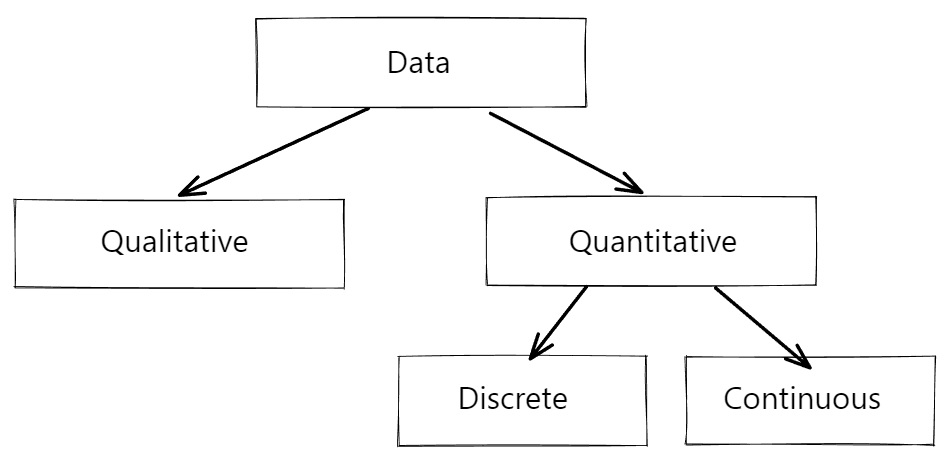
\includegraphics{data.jpg}
There are also different \textbf{levels of measurement}.

\hypertarget{levels-of-measurement}{%
\section{Levels of Measurement}\label{levels-of-measurement}}

The levels of measurement describe how precisely variables are recorded. The different levels of measurement limit which statistics can be used to summarise data and which inferential statistics can be performed. These levels are:

\begin{itemize}
\tightlist
\item
  Nominal
\item
  Ordinal
\item
  Interval
\item
  Ratio
\end{itemize}

\hypertarget{nominal}{%
\subsection{Nominal}\label{nominal}}

\textbf{Nominal data} is a type of data that is used to label variables. It can be categorised but not ranked (eye colour and gender for instance). The values grouped into these categories have no meaningful order. It is not possible to form a meaningful hierarchy of gender or eye colour.

\begin{figure}

{\centering 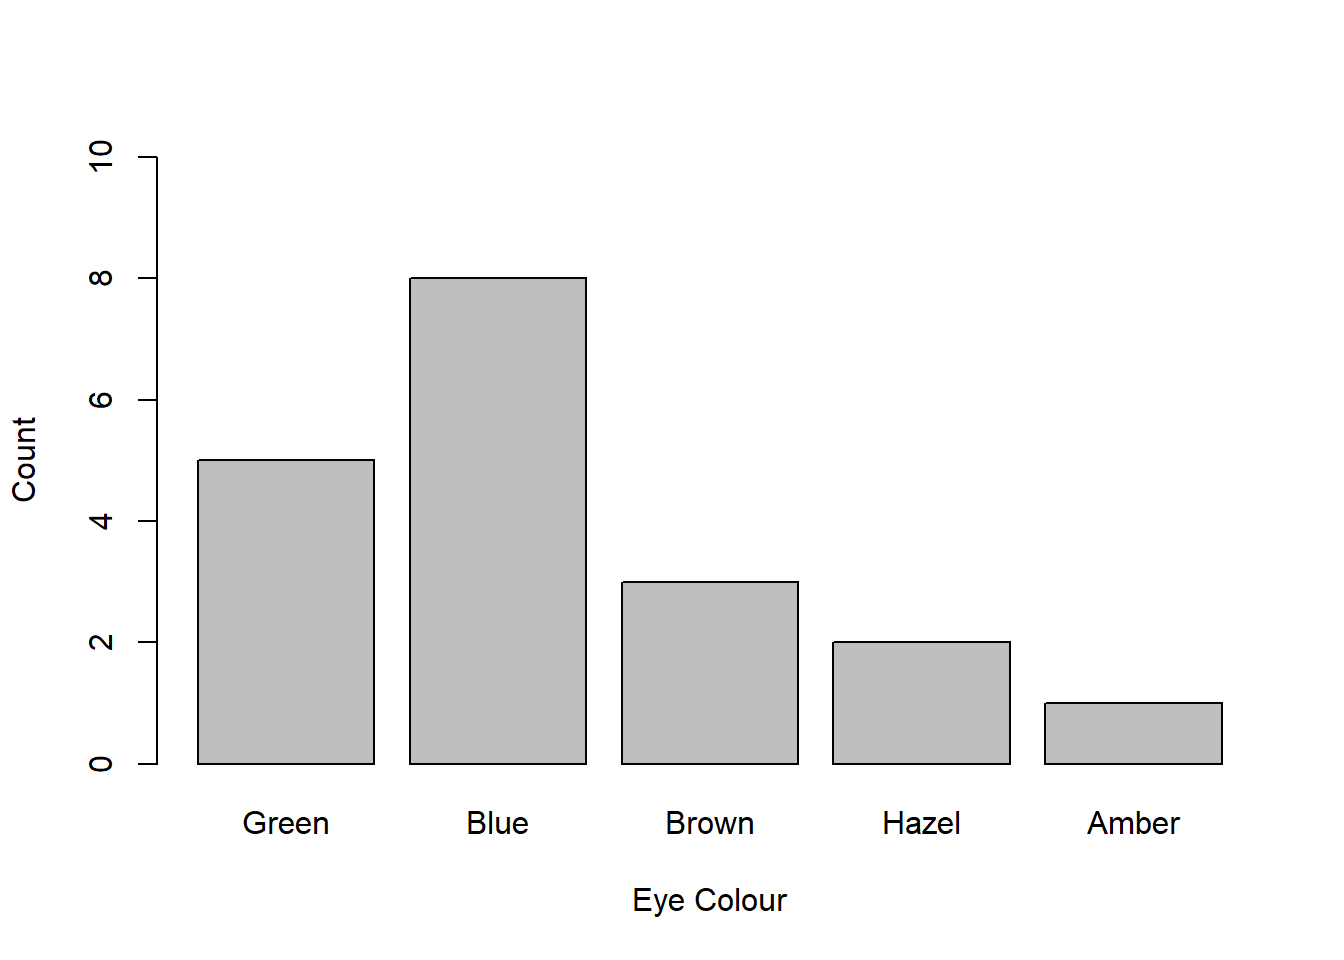
\includegraphics{Bookdown_files/figure-latex/chunk-label-1} 

}

\caption{Eye colour is an example of nominal data.}\label{fig:chunk-label}
\end{figure}

The only measure of central tendency used with nominal data is the mode.

\hypertarget{ordinal}{%
\subsection{Ordinal}\label{ordinal}}

\textbf{Ordinal data} is another type of \textbf{qualitative data} that groups variables into descriptive categories. The categories used for ordinal data are ordered in some kind of hierarchical scale although the distance between those categories may be uneven or even unknown.

\begin{figure}

{\centering 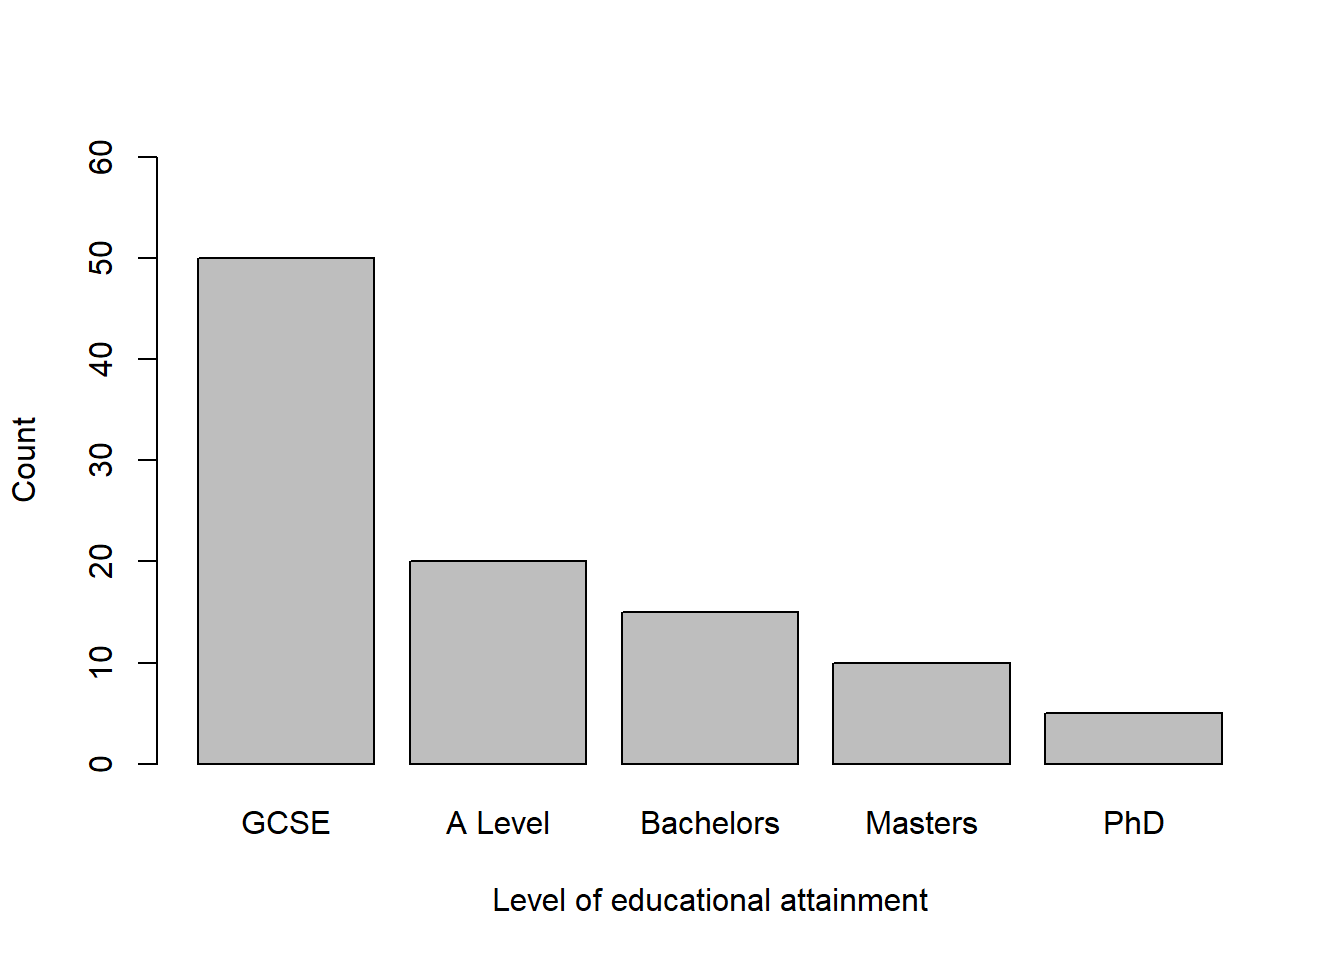
\includegraphics{Bookdown_files/figure-latex/unnamed-chunk-1-1} 

}

\caption{The highest level of educational attainment has a heirarchical scale but the distance between categories is unclear.}\label{fig:unnamed-chunk-1}
\end{figure}

Ordinal variables often include ratings about opinions that can be categorised (strongly agree, agree, don't know, disagree, strongly disagree).

The descriptive statistics which can be used with ordinal data are the mode and the median.

Ordinal data can also be described with a measure of dispersion, namely, range.

\hypertarget{interval}{%
\subsection{Interval}\label{interval}}

\textbf{Interval data} is a type of quantitative data that groups variables into categories. Values can be ordered and separated using an equal measure of distance.

An example of interval level data is temperature data recorded in Celsius or Fahrenheit. The values on either scale are ordered and separated using an equal measure of distance (the distances between notches on a thermometer are always equally spaced).

\begin{figure}

{\centering 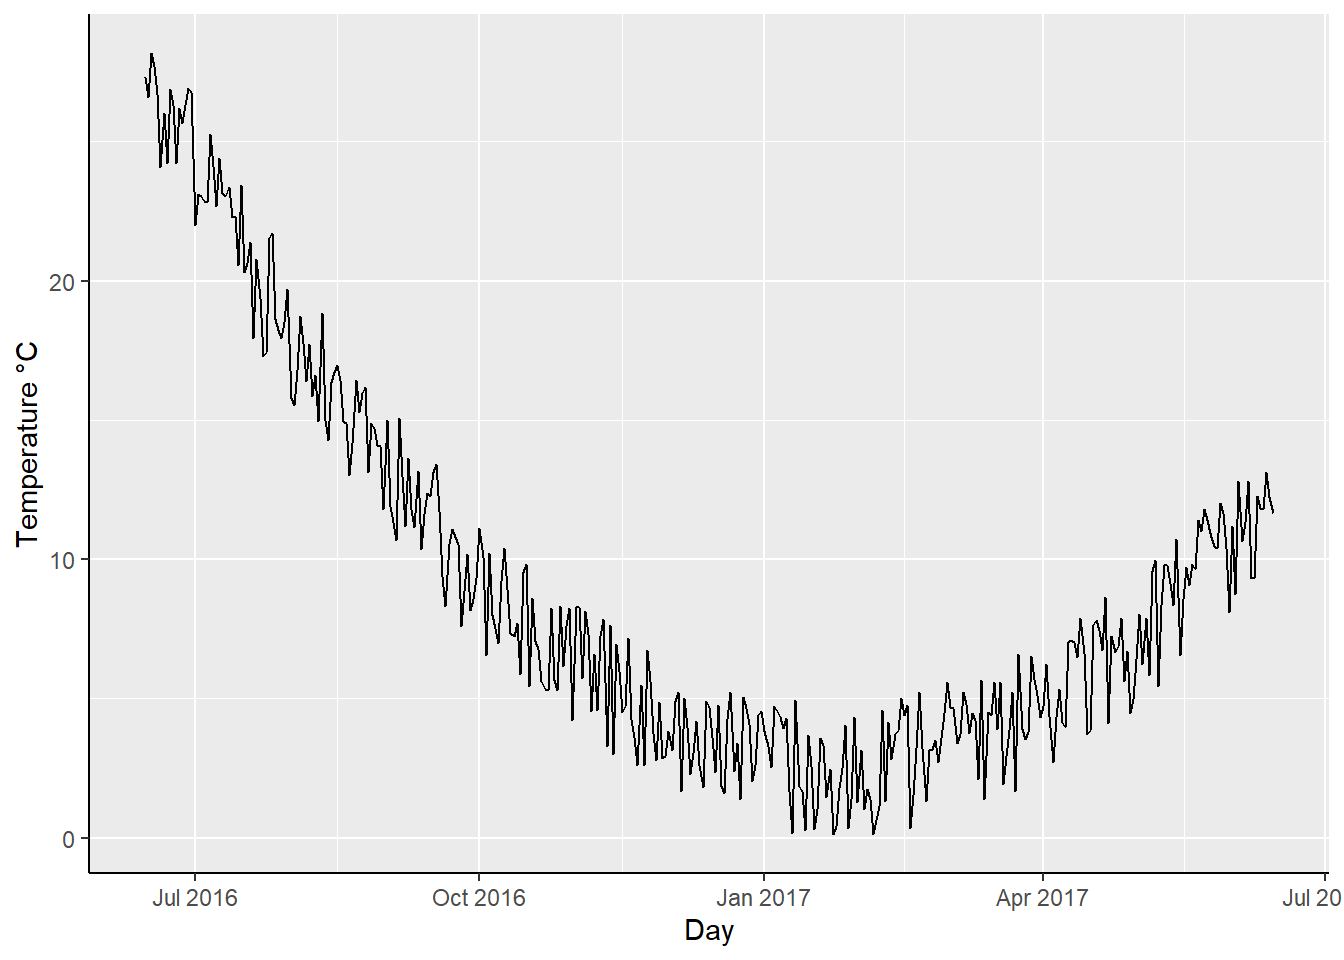
\includegraphics{Bookdown_files/figure-latex/unnamed-chunk-2-1} 

}

\caption{Temperature in Celsius is interval data. The values are ordered and separated by an equal interval. The distance between 0°C and 1°C is the same as the distance between 2°C and 3°C.}\label{fig:unnamed-chunk-2}
\end{figure}

Mathematical operations can be carried out on this type of data, for instance, subtracting one value from another to find the difference. Interval data lacks a \textbf{true zero}.

True zero indicates a lack of whatever is being measured. The Celsius scale doesn't qualify as having a true zero since the zero point in a thermometer is arbitrary. When the Celsius scale was first created by Anders Celsius 0°C was selected to match the boiling point of water and a value of 100 °C was the freezing point of water. The scale was later reversed. Thermometers measure heat and at 0°C there is still heat, maybe not a great deal of it but heat is still measurable meaning 0°C is not a true zero. The thermodynamic Kelvin Scale has a true zero - where particles have no motion and can become no colder (there is a true absence of heat).

A range of descriptive statistics can be used to describe interval data. The measures of central tendency applicable to interval data are the \textbf{mode, median} and the \textbf{mean}. The measures of dispersion applicable to interval data are the \textbf{range, standard deviation} and the \textbf{variance}.

\hypertarget{ratio}{%
\subsection{Ratio}\label{ratio}}

\textbf{Ratio data} is a form of quantitative data. It measures variables on a continuous scale with an equal distance between adjacent values (weight, height). Ratio data has a true zero. Ratio data is the most complex of the four data types.

\begin{figure}

{\centering 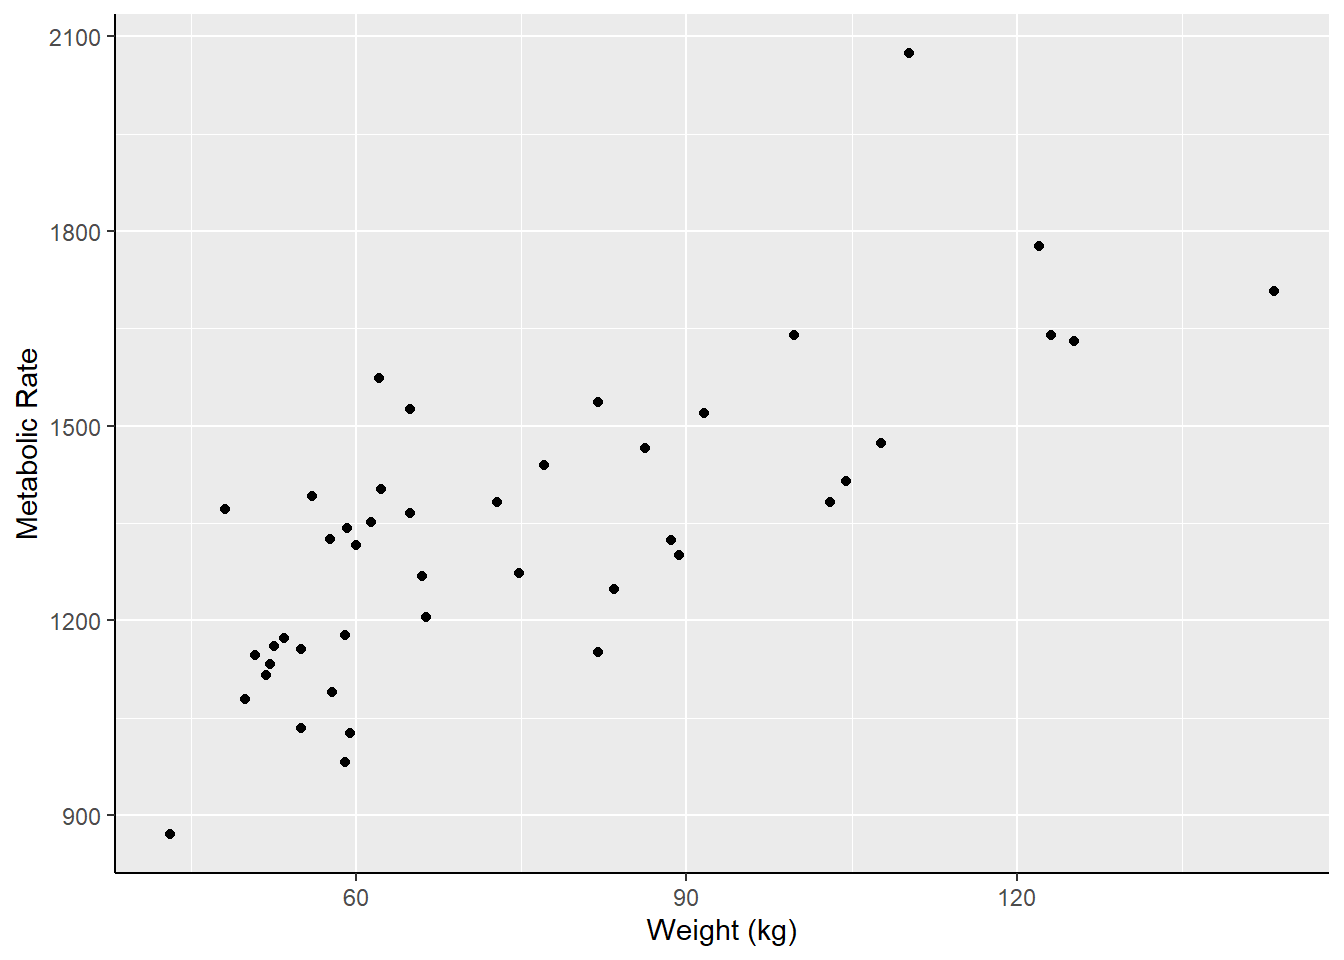
\includegraphics{Bookdown_files/figure-latex/unnamed-chunk-3-1} 

}

\caption{The scatterplot above shows metabolic rate plotted against body weight (kg). These are examples of ratio data. This data comes from the Introduction to Statistics with R (ISwR) library for R.}\label{fig:unnamed-chunk-3}
\end{figure}

Ratio data can be analysed with descriptive statistics including the \textbf{mode, median} and \textbf{mean}. \textbf{Range, standard deviation, variance} and the \textbf{coefficient of variation} can all be used to describe the dispersion of ratio data.

\hypertarget{levels-of-measurement-quiz}{%
\chapter{Levels of Measurement Quiz}\label{levels-of-measurement-quiz}}

\begin{center}\rule{0.5\linewidth}{0.5pt}\end{center}

If you would like to try and test your knowledge of the various levels of measurement outlined in this chapter you can take the \href{https://view.genial.ly/62867083cd8fd700184ca06f/presentation-quiz}{Levels of Measurement Quiz} below. This quiz isn't scored or recorded anywhere.

\hypertarget{describing-data}{%
\chapter{Describing Data}\label{describing-data}}

\begin{center}\rule{0.5\linewidth}{0.5pt}\end{center}

\hypertarget{frequency}{%
\section{Frequency}\label{frequency}}

The \textbf{frequency} of an observation is the number of times it occurs or is recorded.A frequency table, like the one shown below detailing exam grades, is a commonly used method of depicting frequency.

\begin{longtable}[]{@{}rr@{}}
\caption{\label{tab:table2}Frequency Table}\tabularnewline
\toprule
Grade & Frequency \\
\midrule
\endfirsthead
\toprule
Grade & Frequency \\
\midrule
\endhead
A & 15 \\
B & 20 \\
C & 25 \\
D & 21 \\
E & 14 \\
\bottomrule
\end{longtable}

The total of all frequencies so far in a frequency distribution is the \textbf{cumulative frequency}. It is the `running total' of frequencies.

\begin{longtable}[]{@{}rrr@{}}
\caption{\label{tab:table3}Cumulative Frequency Table}\tabularnewline
\toprule
Grade & Frequency & Cumulative Frequency \\
\midrule
\endfirsthead
\toprule
Grade & Frequency & Cumulative Frequency \\
\midrule
\endhead
A & 15 & 15 \\
B & 20 & 35 \\
C & 25 & 60 \\
D & 21 & 81 \\
E & 14 & 95 \\
\bottomrule
\end{longtable}

The \textbf{relative frequency} is the ratio of the category frequency to the total number of outcomes. For grade A, the relative frequency is:

\[ \frac{15}{15+20+25+21+14}=0.16. \]

The table can be extended to include the relative frequency.

\begin{longtable}[]{@{}rrr@{}}
\caption{\label{tab:table4}Relative Frequency Table}\tabularnewline
\toprule
Grade & Frequency & Relative Frequency \\
\midrule
\endfirsthead
\toprule
Grade & Frequency & Relative Frequency \\
\midrule
\endhead
A & 15 & 0.16 \\
B & 20 & 0.21 \\
C & 25 & 0.26 \\
D & 21 & 0.22 \\
E & 14 & 0.15 \\
\bottomrule
\end{longtable}

The \textbf{relative frequency} can be reported as a percentage by multiplying the values by 100\%. For grade A, the relative frequency reported as a percentage is: 100\% x 0.16 = 16\%.

\hypertarget{measures-of-central-tendency}{%
\section{Measures of Central Tendency}\label{measures-of-central-tendency}}

Measures of central tendency help find the middle, or the average, of a data set.The measures of central tendency are the mean, median and mode.

\hypertarget{mean}{%
\subsection{Mean}\label{mean}}

The mean is the sum of the recorded values divided by the number of values recorded.

\hypertarget{example}{%
\subsubsection{Example}\label{example}}

Find the mean of this list of numbers:

\[ 2, 3, 3, 4, 20.\]
\[ \textrm{Mean} = \frac{\textrm{Sum of recorded values}}{\textrm{Number of values recorded}},\]
\[ \textrm{Mean} = \frac{\textrm{2 + 3 + 3 + 4 + 20}}{\textrm{5}},\]
\[ \textrm{Mean} = \frac{\textrm{32}}{\textrm{5}},\]

\[ \textrm{Mean} = 6.4.\]

\hypertarget{median}{%
\subsection{Median}\label{median}}

The \textbf{median} is the middle number in a sorted, ascending or descending, list of values.

If there are an odd number of values the median is simply the middle value.

For an even number of values there will be two values in the center. Those values are summed and divided by two.

The median is sometimes used as opposed to the mean when there are outliers that might skew the average of the values.

\hypertarget{example-1}{%
\subsubsection{Example}\label{example-1}}

Find the median of this list of numbers:

\[ 2, 3, 3, 4, 20.\]

There are 5 values listed in ascending order and the middle value is the third value in the list so the median is 3.

Note: In the previous example the mean was 6.4. It was skewed by the outlier (20). The median remains closer to what might be considered to be the middle of the data set.

\hypertarget{example-2}{%
\subsubsection{Example}\label{example-2}}

Find the median of this list of numbers:

\[ 3, 5, 4, 4, 2, 8, 7, 1.\]

The list should be sorted:

\[ 1, 2, 3, 4, 4, 5, 7, 8. \]

There are an even number of values so there will be two middle values. The middle values are 4 and 4. Sum them and divide by two to get the median: 4.

\hypertarget{mode}{%
\subsection{Mode}\label{mode}}

The mode of a set of data values is the value that appears most often. It is the value that is most likely to be sampled. There can be multiple modes or no modes.

\hypertarget{example-3}{%
\subsubsection{Example}\label{example-3}}

Find the mode of this list of numbers:

\[ 1, 2, 2, 2, 3, 3, 4.\]

A simple way to find the mode is to make a frequency table with the unique values on the left hand side and their frequency on the right hand side. We can tally up how many times each number occurs. Whichever has the greatest frequency is our mode.

\begin{longtable}[]{@{}rr@{}}
\caption{\label{tab:table5}}\tabularnewline
\toprule
Value & Frequency \\
\midrule
\endfirsthead
\toprule
Value & Frequency \\
\midrule
\endhead
1 & 1 \\
2 & 3 \\
3 & 2 \\
4 & 1 \\
\bottomrule
\end{longtable}

The mode is 2.

\hypertarget{example-4}{%
\subsubsection{Example}\label{example-4}}

Find the mode of this list of numbers:

\[ 7, 3, 5, 3, 4, 3, 5, 6, 8, 5.\]

\begin{longtable}[]{@{}rr@{}}
\caption{\label{tab:table6}}\tabularnewline
\toprule
Value & Frequency \\
\midrule
\endfirsthead
\toprule
Value & Frequency \\
\midrule
\endhead
3 & 3 \\
4 & 1 \\
5 & 3 \\
6 & 1 \\
7 & 1 \\
8 & 1 \\
\bottomrule
\end{longtable}

This is \textbf{bimodal}, it has two modes, 3 and 5.

\hypertarget{example-5}{%
\subsubsection{Example}\label{example-5}}

Find the mode of this list of numbers:

\[ 1, 2, 3, 4, 5, 6.\]

\begin{longtable}[]{@{}rr@{}}
\caption{\label{tab:table7}}\tabularnewline
\toprule
Value & Frequency \\
\midrule
\endfirsthead
\toprule
Value & Frequency \\
\midrule
\endhead
1 & 1 \\
2 & 1 \\
3 & 1 \\
4 & 1 \\
5 & 1 \\
6 & 1 \\
\bottomrule
\end{longtable}

Every value is unique and occurs only once so this data has no mode.

\hypertarget{using-excel}{%
\subsection{Using Excel}\label{using-excel}}

It is useful to calculate descriptive statistics by hand for understanding but for larger data sets it is not always possible to arrange data and perform calculations by hand.

Excel has a number of functions designed to perform descriptive statistics.

\textbf{Frequency}

=FREQUENCY(start:end,bins\_array)

The frequency() function will return a frequency table describing your data. It takes two arguments, the first being the array of values and the second being an array describing the upper boundary of the bins used.

\textbf{Average}

=AVERAGE(start:end)

The mean is calculated using the average() function. There are several other functions relating to means: geomean(), harmean() and trimmean(). Take care not to use these as they are quite different from calculating the mean that has been described here.

\textbf{Median}

=MEDIAN(start:end)

The median is calculated using the median() function.

\textbf{Mode}

=MODE.SNGL(start:end)

=MODE.MULT(start:end)

There are several functions for calculating the mode: mode(), mode.sngl() and mode.mult().
mode() was used in Excel 2007 and may still appear as an option in some versions of Excel.
mode.sngl() will return one mode and mode.mult() will return multiple modes (if there are multiple modes).

Neither mode() nor mode.sngl() will warn you if there are multiple modes so mode.mult() is usually the safest option.

\hypertarget{example-6}{%
\subsubsection{Example}\label{example-6}}

In the example below, the variable name is in cell A1 and the values are in cells A2 to A18. To calculate the average, type ``=AVERAGE(A2:A18)'' in another cell. It doesn't matter which cell but in this example A19 has been used. Press enter to return the value.

\begin{figure}
\centering
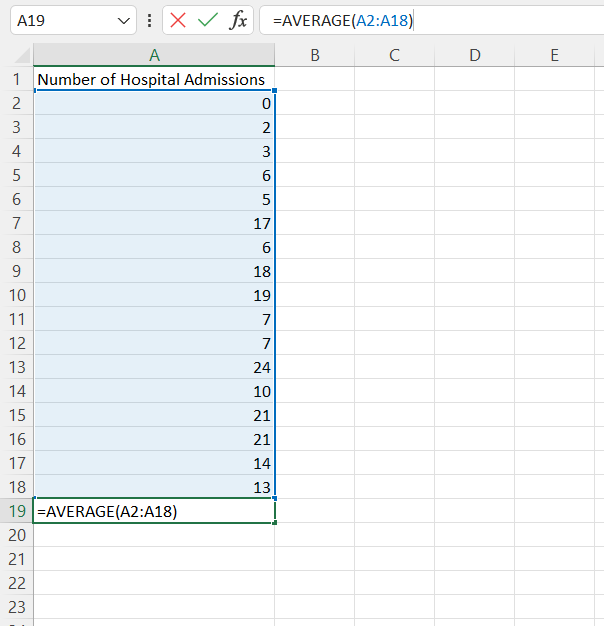
\includegraphics{Excelimage.png}
\caption{Screen shot showing excel spreadsheet with a list of values and the average being calculated using the average() function.}
\end{figure}

\hypertarget{measures-of-dispersion}{%
\section{Measures of Dispersion}\label{measures-of-dispersion}}

\textbf{Dispersion} (or variability) describes how far apart data points lie from each other and the center of a distribution. The \textbf{range, interquartile range, variance} and \textbf{standard deviation} are all measures of dispersion and they describe how far apart data points lie from one another and the center of a distribution.

\hypertarget{range}{%
\subsection{Range}\label{range}}

The range is the difference between the highest and lowest values and is calculated by subtracting the minimum value from the maximum value.

\hypertarget{example-7}{%
\subsubsection{Example}\label{example-7}}

Calculate the range for the following set of numbers:

\[ 23, 42, 75, 19, 74. \]
First, arrange the values in ascending order:

\[ 19, 23, 42, 74, 75. \]
The maximum value is 75 and the minimum is 19.

\[ \textrm{Range}= 75 - 19, \]
\[ \textrm{Range} = 56.\]

\hypertarget{interquartile-range}{%
\subsection{Interquartile Range}\label{interquartile-range}}

The \textbf{interquartile range} (IQR) describes the spread of the middle half of a distribution. How the interquartile range is calculated depends on whether there are an even or an odd number of values in a dataset.

For an even number of values the dataset in split half. The medians for the two new subsets of data are calculated. The positive difference of those medians is the interquartile range.
For an odd number of values either the inclusive or the exclusive method of finding the interquartile range must be used.

\begin{figure}
\centering
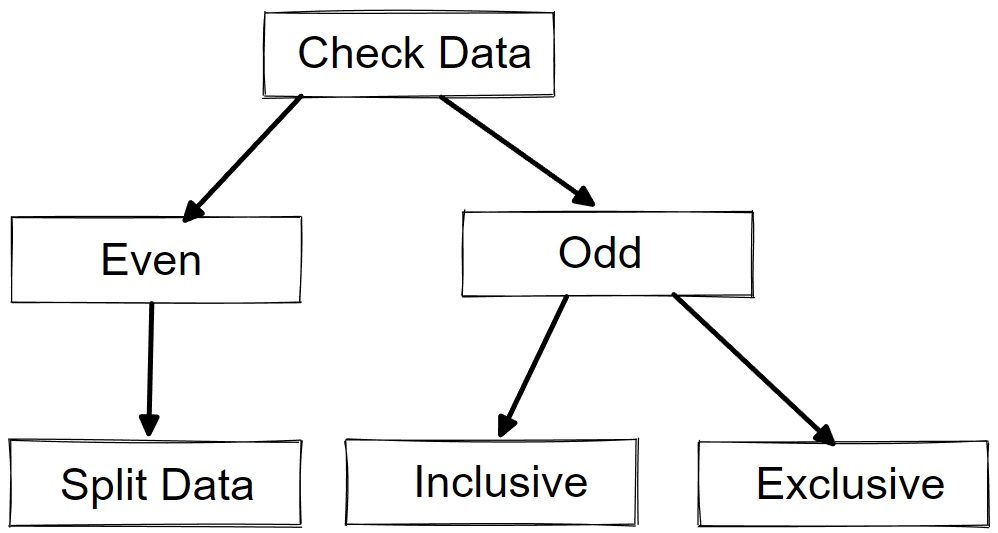
\includegraphics{iqrtree.jpg}
\caption{Tree diagram showing process of deciding how to calculate the IQR}
\end{figure}

The algorithm for the \textbf{exclusive method} is detailed below:

\begin{enumerate}
\def\labelenumi{\arabic{enumi}.}
\tightlist
\item
  Arrange the data in numeric order.
\item
  Remove the median and split the data about its center.
\item
  Find the medians of the two newly appended subsets of data.
\item
  Calculate the difference.
\end{enumerate}

The algorithm for the \textbf{inclusive method} is detailed below:

\begin{enumerate}
\def\labelenumi{\arabic{enumi}.}
\tightlist
\item
  Arrange the data in numeric order.
\item
  Remove the median and split the data about its center.
\item
  Append the two new subsets of data with the median.
\item
  Find the medians of the two newly appended subsets of data.
\item
  Calculate the difference.
\end{enumerate}

\hypertarget{example-8}{%
\subsubsection{Example}\label{example-8}}

\textbf{Even}

Find the interquartile range for the list of numbers below:

\[6, 7, 8, 8, 7, 6, 9, 5, 10, 4. \]
There are an even number of values. Arrange them in numeric order:

\[ 4, 5, 6, 6, 7, 7, 8, 8, 9, 10.\]
Split the values about their center into two sub sets of data.

\[ (4, 5, 6, 6, 7), (7, 8, 8, 9, 10). \]
Find the medians of each of these sub sets. The first subset has a median of 6 while the second has a median of 8.

The interquartile range is:

\[ \textrm{IQR} = 8 - 6 = 2.\]
Note: To calculate the interquartile range the smaller median value is always subtracted from the larger.

\textbf{Odd (Exclusive Method)}

Find the interquartile range for the list of numbers below:

\[2, 3, 2, 4, 3, 5, 4, 4, 2.\]
Arrange the values in numeric order:

\[2, 2, 2, 3, 3, 4, 4, 4, 5. \]
Remove the median (3) and split the data as before:

\[ (2, 2, 2, 3), (4, 4, 4, 5).\]
The interquartile range is:

\[ \textrm{IQR}=\textrm{Median of sub set 2}- \textrm{Median of sub set 1},\]
\[ \textrm{IQR}=\frac{4+4}{2} - \frac{2+2}{2}=\frac{8}{2} - \frac{4}{2} = 4 - 2= 2.\]
\textbf{Odd (Inclusive Method)}

Find the interquartile range of the list of numbers below:

\[ 2, 3, 2, 4, 3, 5, 4, 4, 2.\]
Sort in numeric order as before:

\[2, 2, 2, 3, 3, 4, 4, 4, 5.\]

Split the data as before but append each subset of data with the median (at the end and start of each subset respectively):

\[(2, 2, 2, 3, 3),(3, 4, 4, 4, 5).\]
Find the medians of each of the subsets and calculate the interquartile range. The median of the first subset is 2 and the median of the second subset is 4.

\[ \textrm{IQR} = 4 - 2 = 2 \]

The interquartile range is a useful measure of variability for skewed distributions. It can show where most values lie and how clustered they are. It is useful for datasets with outliers as it is based on the middle half of the distribution and less influenced by extreme values. Exclusive calculations result in a wider interquartile range than inclusive calculations.

\hypertarget{variance-and-standard-deviation}{%
\subsection{Variance and Standard Deviation}\label{variance-and-standard-deviation}}

The standard deviation describes to what extent a set of numbers lie apart (their spread). It is the square root of variance which is also an indicator of the spread of values.

\textbf{Variance}

To calculate the variance:

\begin{enumerate}
\def\labelenumi{\arabic{enumi}.}
\tightlist
\item
  Start by finding the mean of the values in the dataset.
\item
  Find the difference between each recorded value and the mean.
\item
  Square those differences.
\item
  Sum the squared differences.
\item
  Divide the sum by the number of values recorded for population variance or the sum of the number of values minus 1 for sample variance.
\end{enumerate}

\textbf{Standard Deviation}

Taking square root of the variance corrects for the fact that all the differences were squared, resulting in the standard deviation.

The plot below shows three distributions of values, each with a mean of 30 but with different standard deviations. In statistics there is a rule called the empirical rule that states that 68\%, 95\%, and 99.7\% of the values lie within one, two, and three standard deviations of the mean, respectively.

To make sense of this through an example, the plot below shows some simulated data for test scores. Three groups given the same test could achieve the same average score but with greater or lesser spreads of scores.

\begin{figure}

{\centering 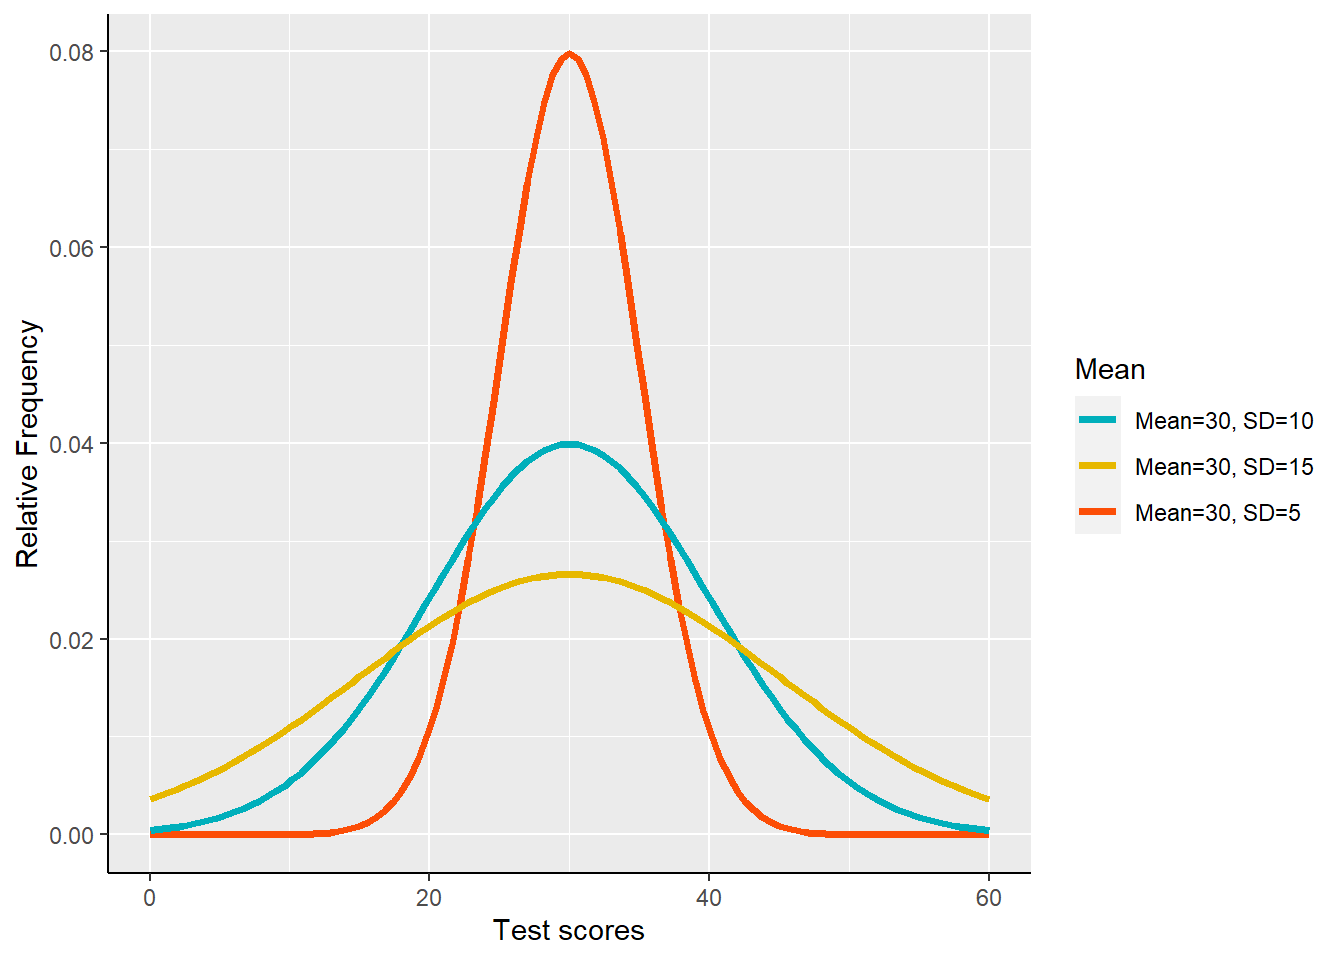
\includegraphics{Bookdown_files/figure-latex/unnamed-chunk-4-1} 

}

\caption{Plot showing several distributions of simulated test score data the same means but differing standard deviations.}\label{fig:unnamed-chunk-4}
\end{figure}

For a mean of 30 and standard deviation of 5: 68\% of the values will lie within the range 25-35.

For a mean of 30 and standard deviation of 10: 68\% of the values will lie within the range 20-40.

For a mean of 30 and standard deviation of 15: 68\% of the values will lie within the range 15-45.

This is particularly clear with a mean of 30 and a standard deviation of 5 as most of the values are tightly packed within the range 25-35.

\hypertarget{example-9}{%
\subsubsection{Example}\label{example-9}}

Calculate the sample estimate of variance and sample estimate of standard deviation for the following list of values:

\[ 2, 4, 4, 5, 6.\]

Start by finding the mean of the values in the dataset:

\[ \textrm{Mean}= \frac{2 + 4 + 4 + 5 + 6}{5}=4.2.\]
Find the difference between each recorded value and the mean.

\begin{longtable}[]{@{}rr@{}}
\caption{\label{tab:table8}}\tabularnewline
\toprule
Value & Difference \\
\midrule
\endfirsthead
\toprule
Value & Difference \\
\midrule
\endhead
2 & 2 - 4.2 = -2.2 \\
4 & 4 - 4.2 = -0.2 \\
4 & 4 - 4.2 = -0.2 \\
5 & 5 - 4.2 = 0.8 \\
6 & 6 - 4.2 = 1.8 \\
\bottomrule
\end{longtable}

Square the differences.

\begin{longtable}[]{@{}rrr@{}}
\caption{\label{tab:table9}}\tabularnewline
\toprule
Value & Difference & Squared Difference \\
\midrule
\endfirsthead
\toprule
Value & Difference & Squared Difference \\
\midrule
\endhead
2 & -2.2 & 4.84 \\
4 & -0.2 & 0.04 \\
4 & -0.2 & 0.04 \\
5 & 0.8 & 0.64 \\
6 & 1.8 & 3.24 \\
\bottomrule
\end{longtable}

Sum the squared differences.

\[\textrm{Sum} = 4.84 + 0.04 + 0.04 + 0.64 + 3.24 = 8.8. \]

Divide the sum by the number of values recorded minus one to get the sample estimate of variance.

\[ \textrm{Variance}_{S} = \frac{8.8}{5-1} = 2.2.\]

To get the sample estimate of the standard deviation take the square root of this value:

\[ \textrm{Standard Deviation}_S = \sqrt{ \textrm{Variance}_{S}} = \sqrt{2.2} = 1.48.\]

\hypertarget{using-excel-1}{%
\subsection{Using Excel}\label{using-excel-1}}

Calculating the variance and standard deviation by hand is a long process and due to the number of steps involved it is prone to error. Excel, SPSS, Python and R all have functions which allow users to calculate these descriptive statives and their use is highly recommended over calculating the statistics by hand.

\textbf{Range}

=MAX(start:end)-MIN(start:end)

\textbf{Standard Deviation}

=STDEV.S(start:end)
=STDEV.P(stard:end)

stdev.s() estimates standard deviation based on a sample. stdev.p() calculates standard deviation based on the entire population given as arguments.

\textbf{Variance}

=VAR.S(start:end)
=VAR.P(start:end)

var.s() estimates variance based on a sample. var.p() calculates variance based on the entire population given as arguments.

\hypertarget{descriptive-statistics-quiz}{%
\chapter{Descriptive Statistics Quiz}\label{descriptive-statistics-quiz}}

\begin{center}\rule{0.5\linewidth}{0.5pt}\end{center}

If you would like to try and test your knowledge of the various levels of measurement outlined in this chapter you can take the \href{https://view.genial.ly/628a683cb8b7d200114d12a0/presentation-quiz-on-measures}{Measures of Central Tendency and Measures of Dispersion Quiz} below. This quiz isn't scored or recorded anywhere.

\hypertarget{comparing-data}{%
\chapter{Comparing Data}\label{comparing-data}}

\begin{center}\rule{0.5\linewidth}{0.5pt}\end{center}

\hypertarget{percentage-change}{%
\section{Percentage Change}\label{percentage-change}}

Percentage change is about comparing old to new values. The formula for calculating a percentage change is given below:

\[ \textrm{Percentage Change} = 100\% \frac{\textrm{New Value} - \textrm{Old Value}}{\textrm{Old Value}}.\]

\hypertarget{example-10}{%
\subsection{Example}\label{example-10}}

What is the percentage change in the population in these three places between 2018 and 2019?

\begin{longtable}[]{@{}rrrr@{}}
\caption{\label{tab:table10}}\tabularnewline
\toprule
Location & 2018 & 2019 & Percentage Change (\%) \\
\midrule
\endfirsthead
\toprule
Location & 2018 & 2019 & Percentage Change (\%) \\
\midrule
\endhead
Somewhere & 50 & 36 & -28 \\
Anywhere & 50 & 50 & 0 \\
Elsewhere & 50 & 58 & 16 \\
\bottomrule
\end{longtable}

Use the formula above to calculate the percentage change for Upper Braniel:

\[ \textrm{Percentage Change} = 100\% \frac{\textrm{New Value} - \textrm{Old Value}}{\textrm{Old Value}},\]

\[ \textrm{Percentage Change} = 100\% \frac{36 - 50}{50} = 100\% \frac{-14}{50} = -28\%.\]
A negative percentage change indicates a percentage decrease while a positive percentage change indicates a percentage increase.

\hypertarget{percentage-point-change}{%
\section{Percentage Point Change}\label{percentage-point-change}}

Note that subtracting one percentage from another gives the percentage point change rather than the percentage change.

\hypertarget{example-11}{%
\subsection{Example}\label{example-11}}

What is the percentage point change in the population in these locations between 2018 and 2019?

\begin{longtable}[]{@{}rrrr@{}}
\caption{\label{tab:table11}}\tabularnewline
\toprule
Location & 2018 & 2019 & Percentage Change (\%) \\
\midrule
\endfirsthead
\toprule
Location & 2018 & 2019 & Percentage Change (\%) \\
\midrule
\endhead
Somewhere & 3.5 & 2.5 & -1 \\
Anywhere & 3.4 & 3.3 & -0.1 \\
Elsewhere & 3.3 & 3.8 & 0.5 \\
\bottomrule
\end{longtable}

\hypertarget{data-visualisation}{%
\chapter{Data Visualisation}\label{data-visualisation}}

\begin{center}\rule{0.5\linewidth}{0.5pt}\end{center}

\hypertarget{data-visualisation-1}{%
\section{Data Visualisation}\label{data-visualisation-1}}

Data visualisation is formally defined as the encoding of data using visual cues such as variations in the size, shape and colour of geometric objects (points, lines, bars). The encoding is generally informed by the relationships within the data.

In the bar chart example below the frequencies of different eye colours have been mapped to the heights of the bars.

\begin{figure}

{\centering 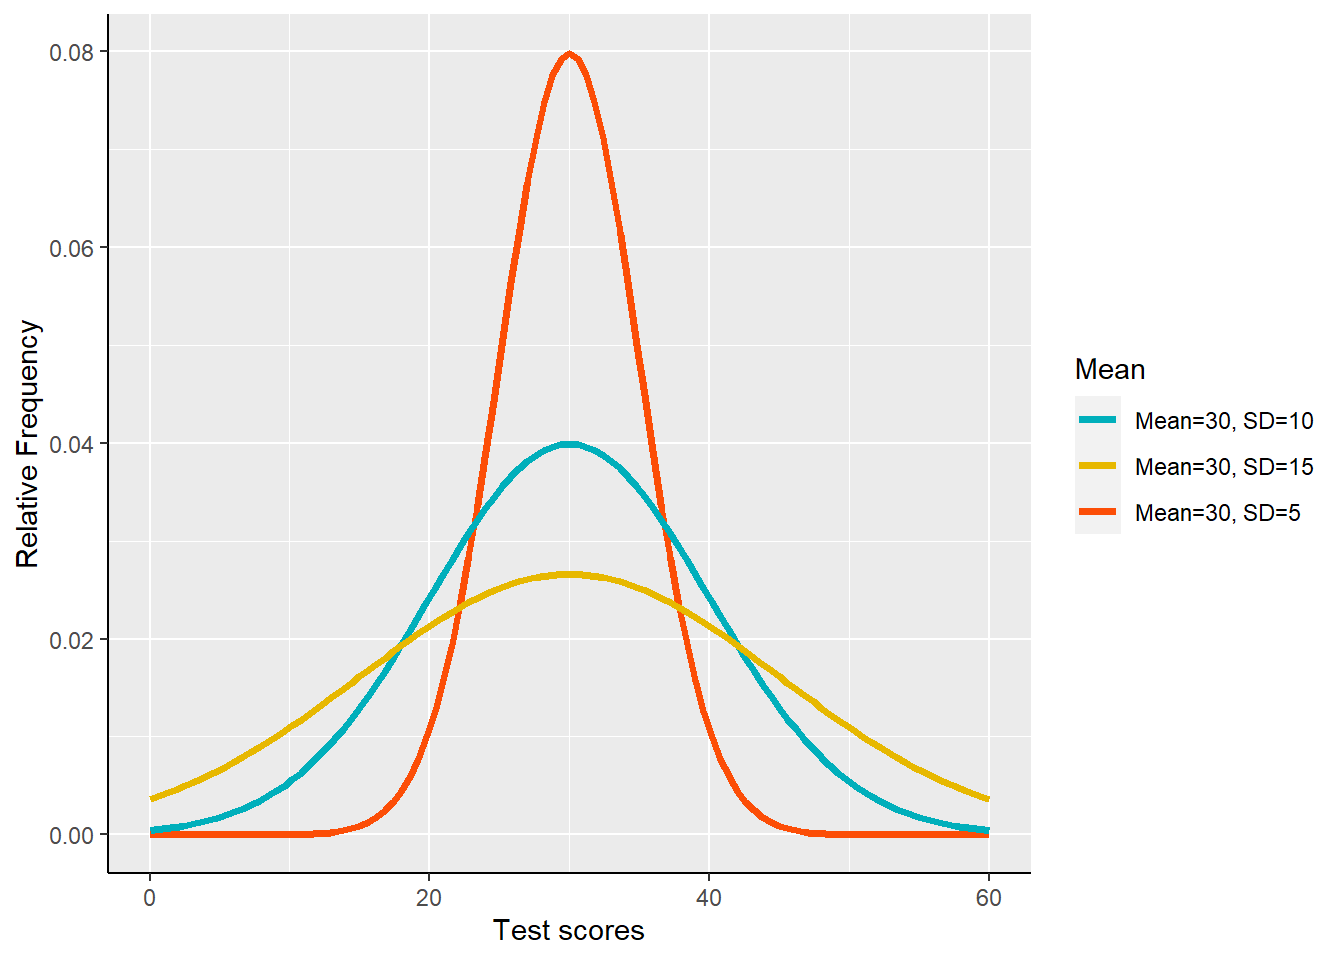
\includegraphics{Bookdown_files/figure-latex/unnamed-chunk-5-1} 

}

\caption{The frequency of each observation has been mapped to the height of the bars in the visual.}\label{fig:unnamed-chunk-5}
\end{figure}

\hypertarget{visual-cues}{%
\section{Visual Cues}\label{visual-cues}}

Whether data is visualised using points, lines, bars or something else entirely is largely determined by the relationships within the data. Some of the visual cues and relationships used to inform data visualisation are shown below.

The illustration above shows some of the visual cues used to encode data. Magnitudes are typically mapped to sizes of objects. Colour is often used to represent quantities or highlight data. Shapes can be used to represent qualitative data.

\hypertarget{relationships-in-data}{%
\section{Relationships in Data}\label{relationships-in-data}}

The \href{https://analysisfunction.civilservice.gov.uk/policy-store/data-visualisation-charts/\#section-9}{Government Statistical Service} has produced guidance on the relationships in data and how they inform chart choices. The guidance can be useful and some of the key points are summarised below.

\hypertarget{frequency-distributions}{%
\subsection{Frequency Distributions}\label{frequency-distributions}}

Histograms and bar charts are useful for showing category frequencies. Population by age band for instance could be visualised using a histogram or bar chart. A boxplot can also be useful in visualising additional descriptive statistics such as the mean, median, quartiles, outliers and the range.

\begin{figure}

{\centering 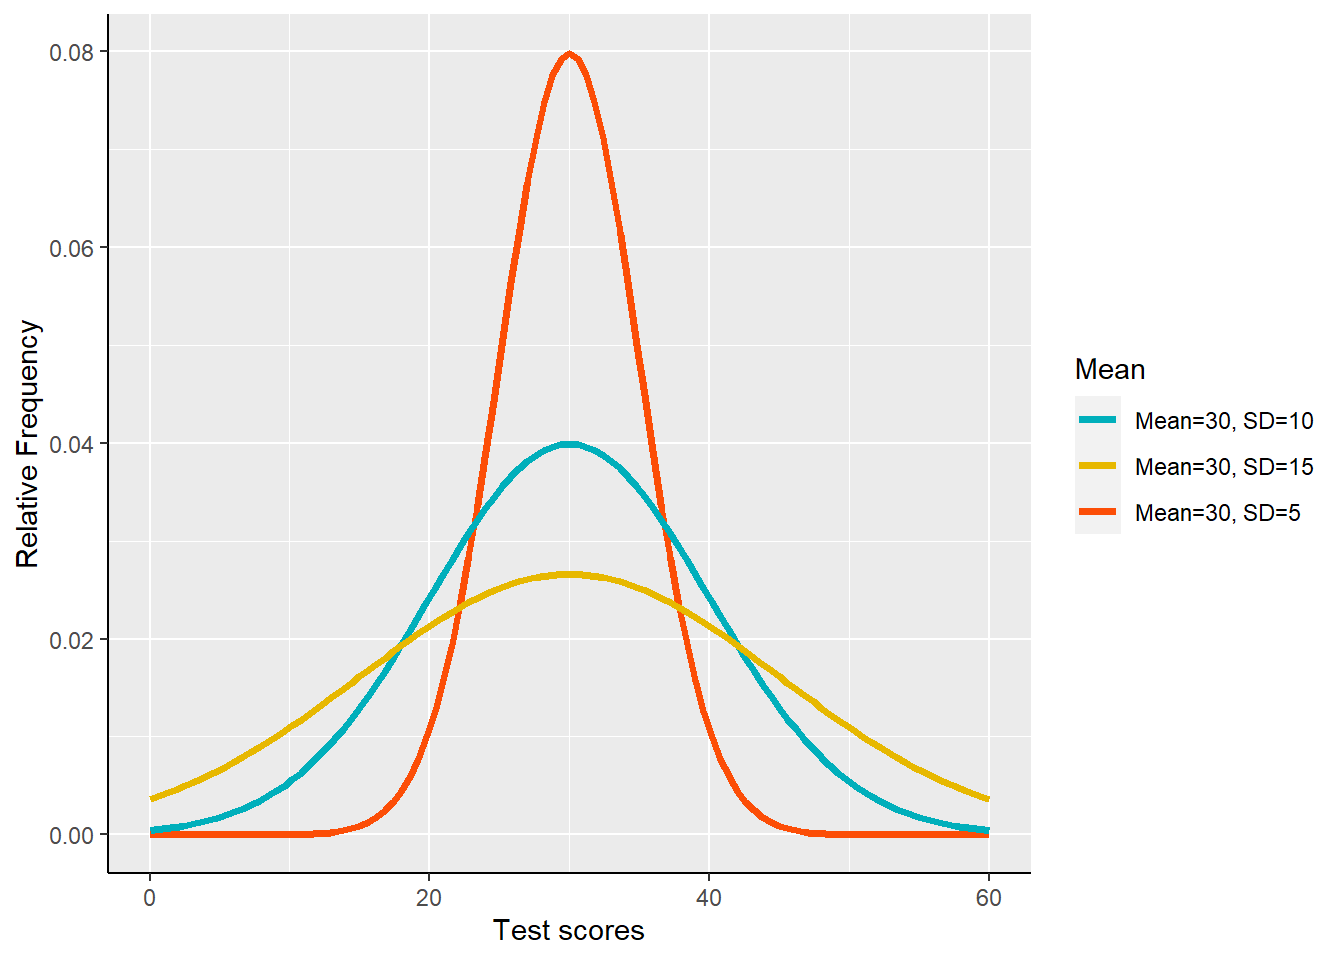
\includegraphics{Bookdown_files/figure-latex/unnamed-chunk-6-1} 

}

\caption{Simulated weight data illustrating the use of a histogram.}\label{fig:unnamed-chunk-6}
\end{figure}

\hypertarget{time-series}{%
\subsection{Time Series}\label{time-series}}

A line chart is often used to demonstrate the trend of a variable over some time period. For instance, temperature over time can be visualised with a line chart.

\begin{figure}

{\centering 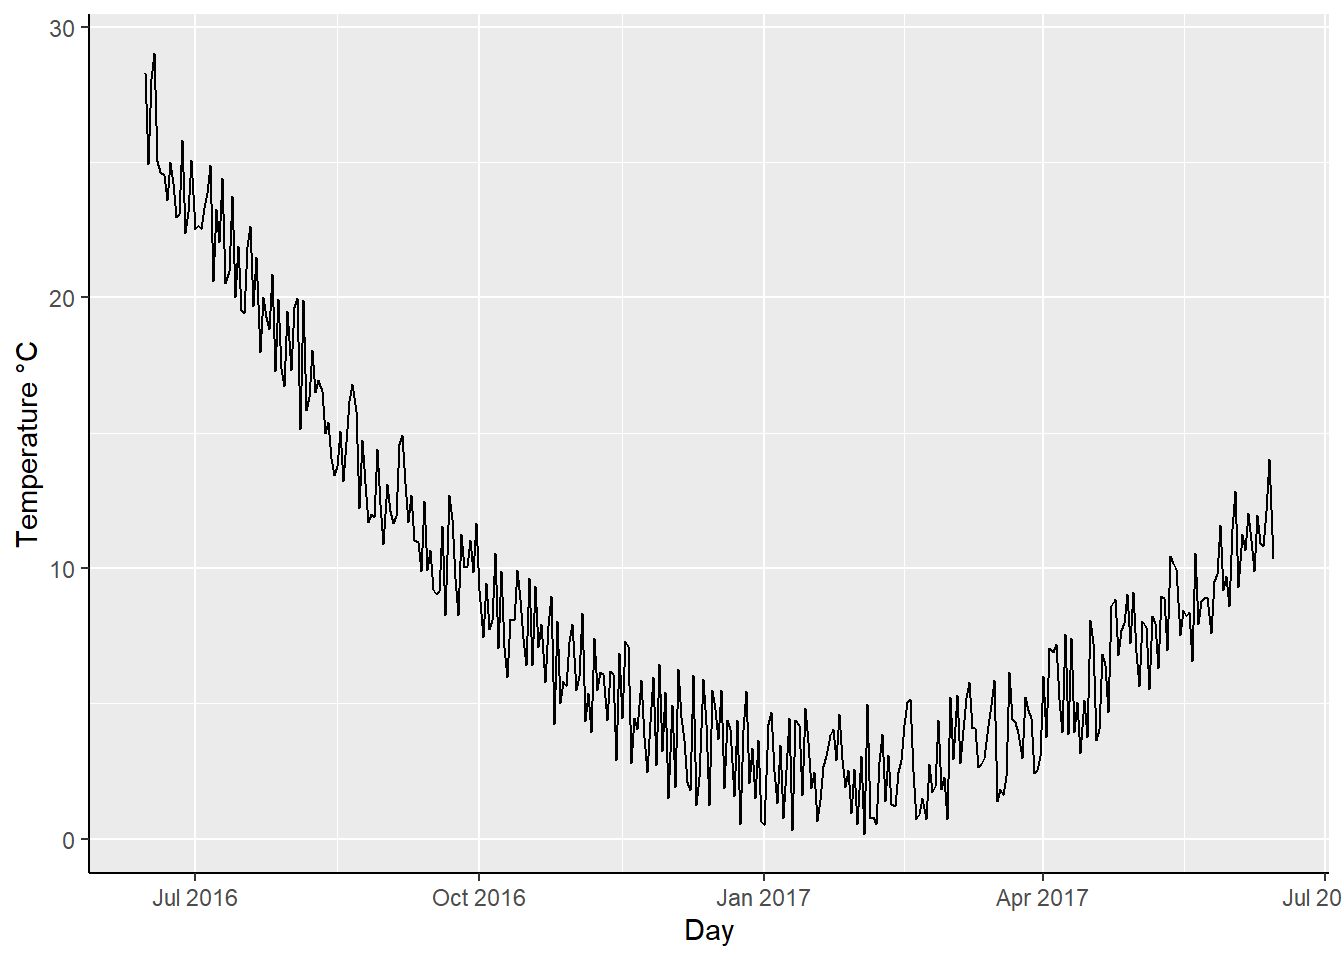
\includegraphics{Bookdown_files/figure-latex/unnamed-chunk-7-1} 

}

\caption{Simulated temperature data.}\label{fig:unnamed-chunk-7}
\end{figure}

\hypertarget{rankings}{%
\subsection{Rankings}\label{rankings}}

Data that is ranked usually consists of categories presented in ascending or descending order. A bar chart may be used to show the comparisons between the different categories. Sometimes, change in ranking over time is shown through slope charts but usually only when comparing a start date and an end date without consideration for the time period in between.

\begin{figure}

{\centering 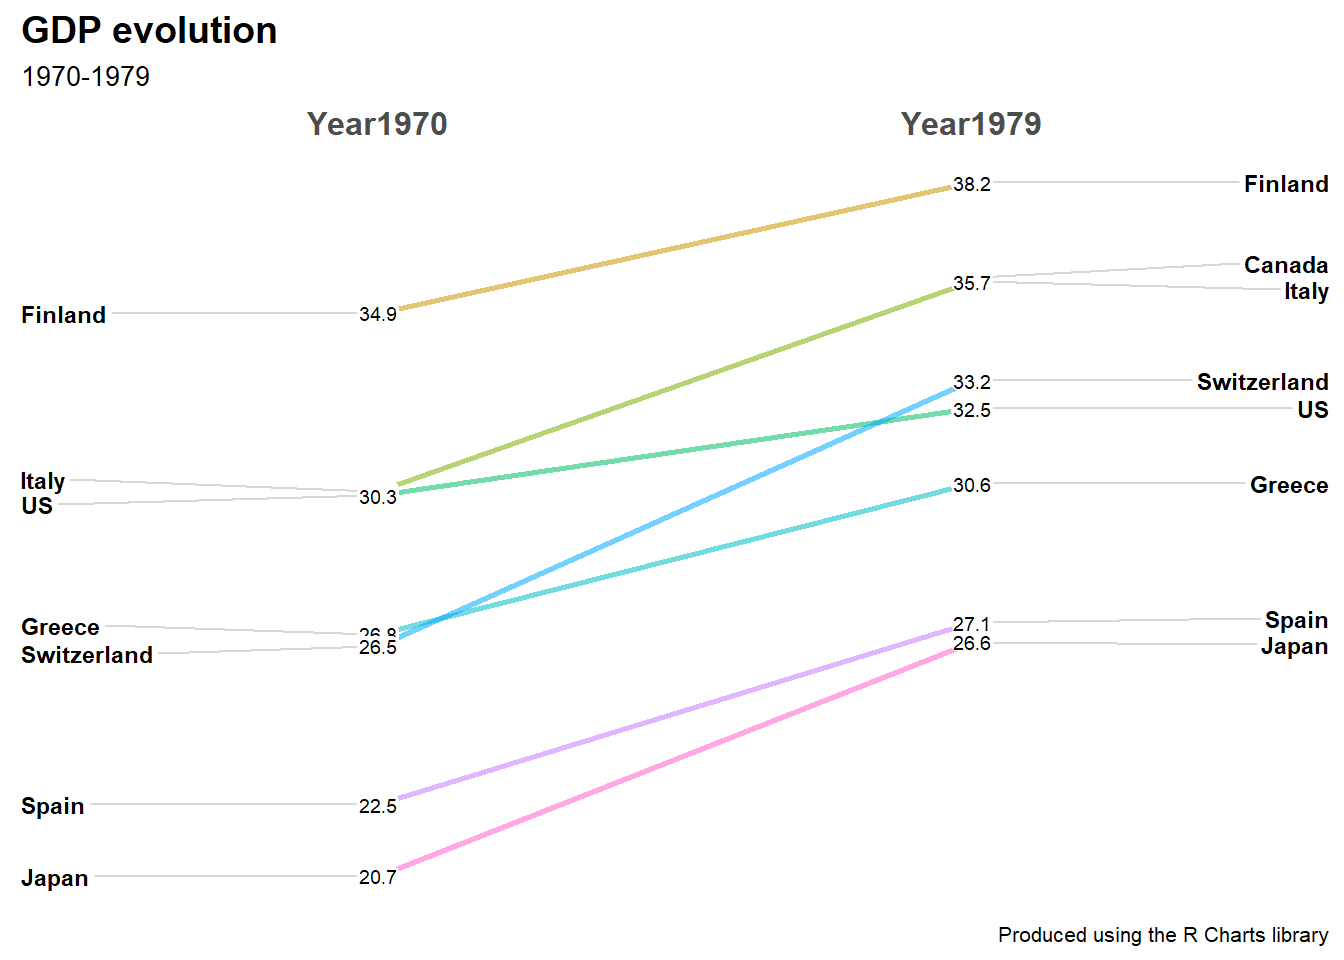
\includegraphics{Bookdown_files/figure-latex/unnamed-chunk-8-1} 

}

\caption{Slope chart showing changes in GDP between 1970 and 1979.}\label{fig:unnamed-chunk-8}
\end{figure}

\hypertarget{deviation}{%
\subsection{Deviation}\label{deviation}}

Deviation from a reference value can be shown through bar charts.

\hypertarget{correlation}{%
\subsection{Correlation}\label{correlation}}

Correlation is usually visualised using scatterplots. Scatterplots are a good way to show comparisons between observations of two variables to determine if there is some correlation because it quickly becomes apparent if there is correlation between the variables or not.

\begin{figure}

{\centering 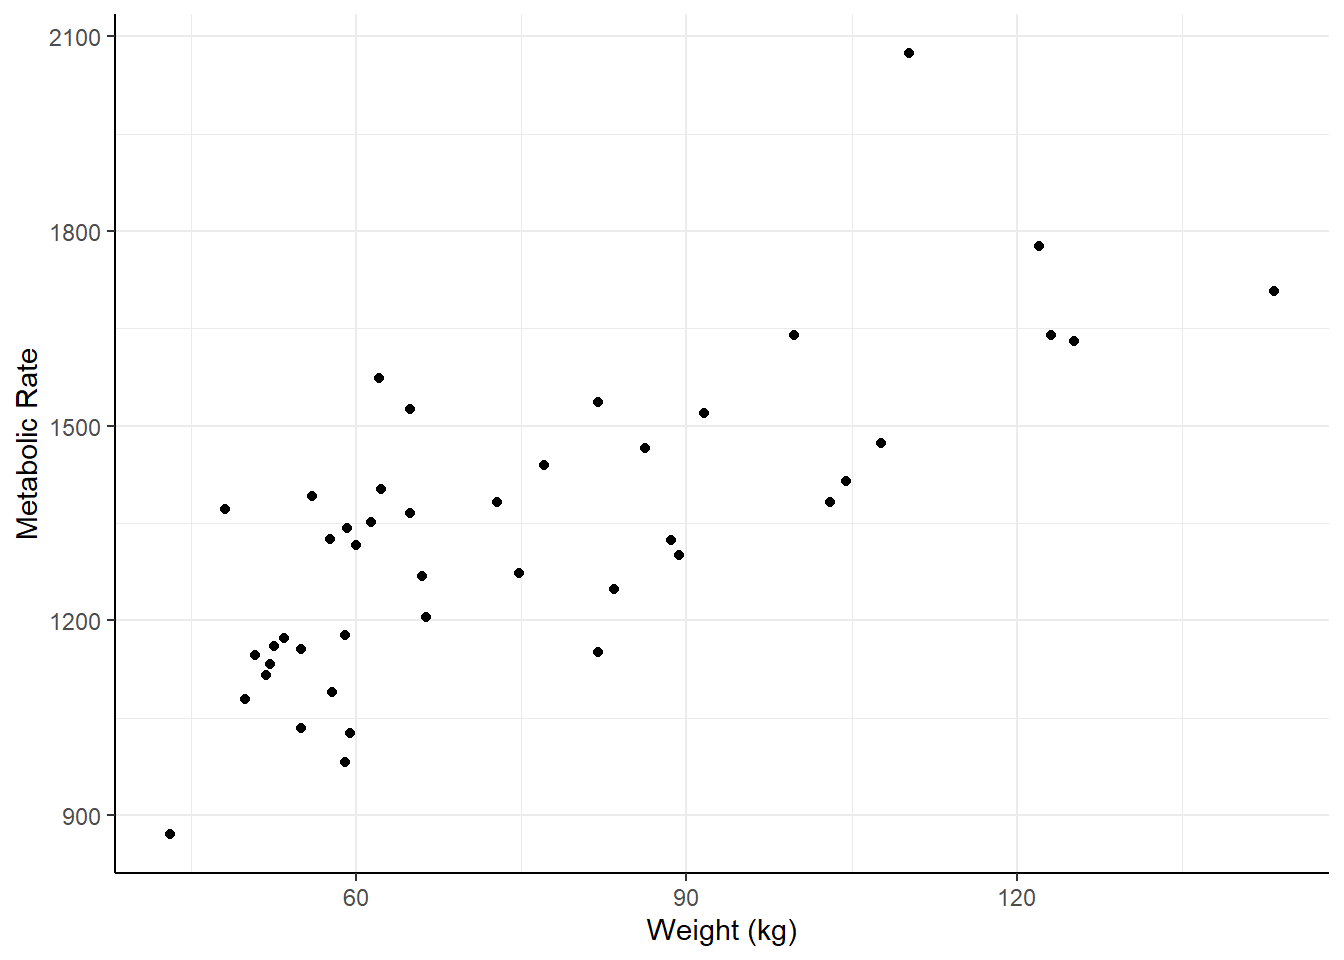
\includegraphics{Bookdown_files/figure-latex/unnamed-chunk-9-1} 

}

\caption{The scatterplot above shows metabolic rate plotted against body weight (kg). This is an example of correlation. This data comes from the Introduction to Statistics with R (ISwR) library for R.}\label{fig:unnamed-chunk-9}
\end{figure}

\hypertarget{magnitude}{%
\subsection{Magnitude}\label{magnitude}}

Comparing differences in the magnitudes of values often relies on bar charts. Comparing the total number of research papers by journal for insance.

\hypertarget{spatial}{%
\subsection{Spatial}\label{spatial}}

Cartograms and heat mapping are common ways to show differences between geographical regions.

\hypertarget{why-visualise-data}{%
\section{Why Visualise Data?}\label{why-visualise-data}}

In general, people are better at recognising differences in shapes, colours and sizes than they are at identifying the number of times a value occurs or the differences between values in a large excel spread sheet. For this reason data visualisation can be used to find errors in data quickly. It's much easier to recognise an anomalous value on a bar chart than in an Excel spread sheet. Data visualisation can also be used to see patterns that are difficult to determine by looking at raw data.
Data visualisation can also be used to:

\begin{itemize}
\tightlist
\item
  Answer research questions.
\item
  Discover new research questions.
\item
  Explain complex relationships in data visually.
\item
  Aid in decision making.
\item
  Engage and inform.
\end{itemize}

\hypertarget{data-visualisation-tools}{%
\section{Data Visualisation Tools}\label{data-visualisation-tools}}

New programming languages and software products have made data analysis and visualisation vastly more accessible. In addition, many of these facilitate dynamic or interactable visualisations. There is an ever expanding ecosystem of data visualisation tools (many of which have been used in this document) including:

\begin{itemize}
\tightlist
\item
  \textbf{Excel} and \textbf{SPSS} produce high quality visualisations and while dynamic visuals are not their focus they are often the simplest and most time efficient option for visualising data.
\item
  \textbf{Genially} is an online tool for creating interactive and animated content that is particularly effective for presentations.
\item
  \textbf{Tableau} and Power BI are visual analytics platforms which are well suited to the development of dashboards to visualise complex interconnected data sets.
\item
  \textbf{Flourish} can be used to produce interactive visuals although its functionality is more limited than Power BI or Tableau.
\item
  \textbf{Javascript} facilitates data visualisation through its D3 library. D3 has a steep learning curve as it requires JavaScript skills to use it effectively however it offers a greater degree of customisation and a broader spectrum of visualisation options as a result.
\item
  \textbf{Python} libraries such as Matplotlib, Seaborn and Plotly can also be used to visualise data. The learning curve is steep as it requires programming skills to use Python effectively however Python offers customisation options that are not available in Excel or Power BI.
\item
  \textbf{R} is another useful tool with libraries such as ggplot2 which can be used to visualise data. This is the programming language used to develop this resource and many of the visualisations throughout.
\end{itemize}

\hypertarget{dynamic-visualisations-dashboards}{%
\section{Dynamic Visualisations (Dashboards)}\label{dynamic-visualisations-dashboards}}

There are a number of considerations when developing dynamic data visualisations (sometimes called dashboards) as not all data visualisations need to be dynamic.

Considering the audience, objectives and what visuals will be most appropriate to communicate data can help in determining whether a dynamic or interactive visualisation is needed.

Dashboard style visualisations are best suited to data reporting where there is a need to repeatedly produce the same visuals or reports either daily, monthly, quarterly or annually.

Power BI is well designed for these types of visualisation requirements as it offers automation options enabling data sets to be refreshed at regular time intervals.
Automation can be as simple as setting a refresh time in the Power BI dashboard and manually updating the excel file it stores in memory or it can be more complex and involve using programming languages to make API calls and perform automated calculations.

Producing dynamic visualisations is often considerably more time expensive than producing static visuals and time constraints should be considered before developing a dashboard visualisation.

\hypertarget{best-practice}{%
\subsection{Best Practice}\label{best-practice}}

GSS have produced \href{https://gss.civilservice.gov.uk/policy-store/top-tips-for-designing-dashboards/}{guidance on designing dashboards} that covers most aspects of dashboard design. The content below summarises some of the key points in this guidance.

\textbf{Consider Audience and User Needs}

Consider the user needs and whether a dashboard is really needed. Often the simplest solution (bar charts drawn in Excel or SPSS) is the best. Consider the visuals used and whether they're the best way to communicate the data. Sometimes tables or even text can communicate data better than a visual.

\textbf{Guidance}

Providing guidance on how to use a dynamic visual or dashboard is important as many users will not be familiar with interactive dashboards. Guidance can be provided through supplementary documentation, blog text if the visual is being embedded, or it can be provided through tool tips and information pages in the dashboard itself.

\textbf{Streamline Content}

When adding any new data or visuals it is important to ask whether it adds value. Try to group related content and streamlining the content to guide the users through the data.

\textbf{Automate }

Automation can be simple or complex, it can be achieved by setting a refresh date in a Power BI dashboard. It can also involve the use of programming languages to make API calls, web scrape data and perform calculations. Automation typically results in less manual updating and a reduced chance of error and can make the management of the product less resource intensive. It's important to note that automation does not necessarily mean less work, the scripts used to automate processes will need to be updated as languages are developed and updated over time.

\textbf{Consider Design Principles}

Give your dashboard a header and dedicated areas for visuals. Consider other dashboards you have seen in the past and draw inspiration from web design. Most websites have a navigation bar at the top, lists with filters along the left or right hand side and content in the center of the page. Think about things like symmetry, flow and a consistent style or layout. Use white space where possible and try to avoid cluttered visualisations.

\textbf{Ensure Accessibility}

Ensure your product is accessible by checking the colour contrast ratios of text and including alt text in your visualisations where possible. Ensure the fonts are large enough to read and avoid using multiple fonts.

\hypertarget{power-bi}{%
\chapter{Power BI}\label{power-bi}}

\hypertarget{introduction}{%
\section{Introduction}\label{introduction}}

\textbf{Power BI} is part of the \textbf{Microsoft Power Platform} which includes other packages such as Power Automate. Power BI is split into several components: Power BI Desktop, Service (an online SaaS - Software as a Service), Gateway, Report Server, Premium, Visuals Marketplace and Mobile Apps. The primary focus of Power BI is business intelligence but Power BI can be used for more than standard reporting of data with line charts and bar charts. It can also be used in conjunction with Python and R to create complex custom visuals or it can be used to create and train \href{https://docs.microsoft.com/en-us/power-bi/connect-data/service-tutorial-build-machine-learning-model}{machine learning models}. Power BI can even be used to \href{https://docs.microsoft.com/en-us/power-bi/connect-data/desktop-connect-to-web-by-example}{web scrape data}.

With Power BI Desktop, you can connect to different data sources, transform those data sources through queries, build data models and create visualizations and reports or dashboards for different audiences. Reports and dashboards can be published to the Power BI Service where you can share your reports with other users or a wider audience.

This document is intended to provide a broad overview of the features of Power BI Desktop reports to provide the reader with the necessary tools to start learning and exploring Power BI for themselves. It covers the basics such as importing data, transforming data, visualizing data, using slicer visuals, navigation and basic UI design.

\hypertarget{getting-started}{%
\subsection{Getting Started}\label{getting-started}}

To download Power BI Desktop, go to the Power BI Desktop download page and select \textbf{Download Free}. You can also download Power BI Desktop from the Power BI service. Select the \textbf{Download} icon in the top menu bar, and then select Power BI Desktop.

Once you launch Power BI Desktop you will be welcomed by the \textbf{Start screen}. Here, you can get data sources for your reports, watch video tutorials, check updates and visit the Power BI forums. For now, select the \textbf{close} icon to close the Welcome screen to see the main interface (Figure 1 below).

\begin{figure}
\centering
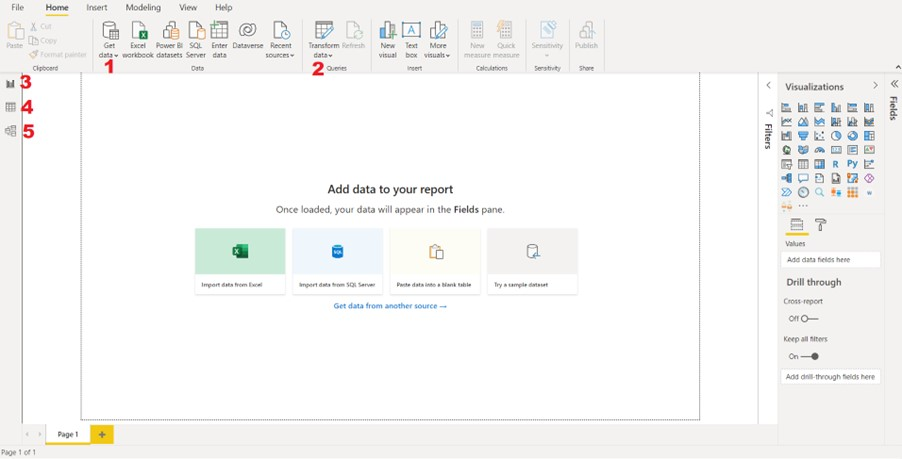
\includegraphics{bi1.jpg}
\caption{Screenshot of the Power BI User Interface.}
\end{figure}

The image above shows some of the most important features in Power BI Desktop.

\begin{enumerate}
\def\labelenumi{\arabic{enumi}.}
\item
  \textbf{Get data}: This is used for selecting, connecting to and configuring the data sources that will be used in a report or dashboard. A single data source can be used or multiple can be used. When a data source is selected Power BI will provide you with an option to either load the data or transform it. It's worth noting that data source will be stored in Power BI's internal memory, so the more data sources you connect to and the larger those sources are the slower your report/dashboard will run.
\item
  \textbf{Transform data}: This is used to launch the Power Query Editor. The Power Query Editor is where data can be transformed. Transformation usually refers to dealing with missing values or cleaning the data before analysis. The Power Query Editor is a useful tool when working with data sets which need to be cleaned. Working with Power Query Editor is similar to working with Excel and often it is useful to switch between the two as some transformations will be easier in one than the other.
\item
  \textbf{Report View or canvas}: The report view icon opens the report view canvas which is used for selecting and designing data visualizations. This is the default view open when Power BI is launched.
\item
  \textbf{Data View}: The data view allows you to view all the data available in your report. This view looks similar to an Excel spreadsheet but it is read only. It is useful to quickly check data types, validate data and make small changes to your data source - such as changing a data type or the format of a variable.
\item
  \textbf{Model View or Relationship View}: The relationship or model view allows you to set relationships between data sources. Relationships occur where two or more data sources are linked together by related data (a shared variable like `year' for instance).
\end{enumerate}

\hypertarget{excel-as-a-data-source}{%
\subsection{Excel as a Data Source}\label{excel-as-a-data-source}}

We're going to use a dummy dataset health\_data.xlsx included in the \href{https://github.com/aamcmurray/BookTest/blob/main/health_data.xlsx}{repository used to host this guide}. Download and save the dataset in a folder you can easily locate.

To use Excel data sets as a source, open the Power BI Desktop. Under the \textbf{Home ribbon} find \textbf{Get Data}. Selecting the down arrow next to the Get Data button will show the most common connectors used but clicking the button itself will provide a full list of all available connectors. The list is extensive and Power BI can connect to a wide array of data sources including .csv files, .xlsx and .txt files. Power BI also supports SQL database connections. Whether you click the Get Data button or the arrow you will see Excel at the top of the resulting list. Click \textbf{Excel Workbook} and then click Connect. Navigate to your data source.

Once selected you will see two separate spreadsheets you can choose from.

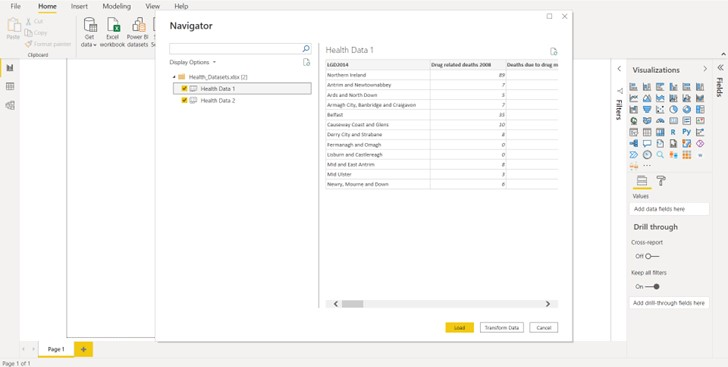
\includegraphics{bi2.jpg}
Clicking once on the spreadsheet name will let you preview the data while clicking on the \textbf{checkbox} next to the name will include it as part of the data import. Here we have two sheets, Health Data 1 which contains data relating to drug related deaths and deaths due to drug misuse and Health Data 2 which contains population data. This data needs to be cleaned before we can use it so tick both the boxes and then press the \textbf{Transform Data} button on the bottom of the panel. This launches the \textbf{Power Query Editor}. You can also clean your data in Excel then simply press the Load button but some data sets would be too difficult to transform in Excel.

When the Power Query Editor loads you will notice it has its own environment.

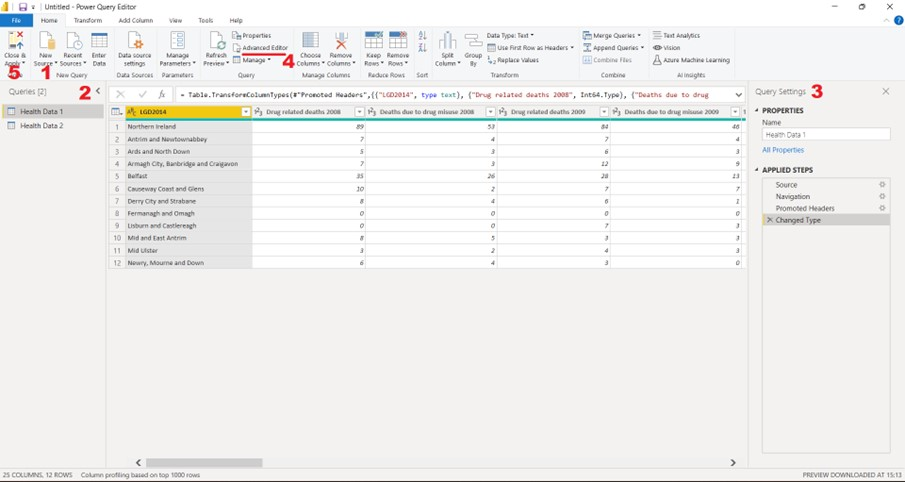
\includegraphics{bi3.jpg}
There are a number of features in the Power Query Editor to take note of:

\begin{enumerate}
\def\labelenumi{\arabic{enumi}.}
\item
  \textbf{New Source}: This launches the same interface as the Get Data button.
\item
  \textbf{Queries Pane}: The queries pane is a list of all the queries that you have connected to.
\item
  \textbf{Query Settings}: Within this pane you can see the complete history of transformations that have been applied to your query. You can also rename the query. This history is useful for several reasons. From here you can rename a query, or click the `x' beside a query to remove a query, and reorder queries by clicking and dragging them into different positions.
\item
  \textbf{Advanced Editor}: Power Query Editor uses a programming language informally known as M in the background and when you click any button in the Power Query GUI some M code is generated in the background corresponding to what has been done. By launching the Advanced Editory you can see the M query that is automatically written for you by the Power Query Editor.
\item
  \textbf{Close and Apply}: Choosing this option will save your transformations, close the Power Query Editor and load the transformed data into the data model.
\end{enumerate}

The Power Query Editor allows you to transform the data with step-by-step instructions for adjusting the data. Transforming the data this way \textbf{does not affect the original data source}, only this particular view of the data. Data transformation includes a range of processes including: renaming columns or tables, removing rows, replacing missing data entries or changing data types. Power Query Editor records the steps taken to transform the data sequentially under \textbf{Applied Steps} in the \textbf{Query Settings} pane. If you make a mistake or transform the data in a way you aren't happy with you can simply cancel the transformation by clicking the \textbf{X} that appears beside it in \textbf{Applied Steps}.

\hypertarget{data-transformation-basics}{%
\section{Data Transformation Basics}\label{data-transformation-basics}}

In its current format the data contained in Health Data 1 will be hard to visualize in Power BI. We essentially have two data sets in one and quantitative data is tied up with qualitative data (Drug related deaths 2008). Ideally, we would like the data to look like this:

\begin{longtable}[]{@{}
  >{\raggedleft\arraybackslash}p{(\columnwidth - 6\tabcolsep) * \real{0.3256}}
  >{\raggedleft\arraybackslash}p{(\columnwidth - 6\tabcolsep) * \real{0.2558}}
  >{\raggedleft\arraybackslash}p{(\columnwidth - 6\tabcolsep) * \real{0.2093}}
  >{\raggedleft\arraybackslash}p{(\columnwidth - 6\tabcolsep) * \real{0.2093}}@{}}
\caption{\label{tab:table12}}\tabularnewline
\toprule
\begin{minipage}[b]{\linewidth}\raggedleft
Location
\end{minipage} & \begin{minipage}[b]{\linewidth}\raggedleft
Dataset
\end{minipage} & \begin{minipage}[b]{\linewidth}\raggedleft
Year
\end{minipage} & \begin{minipage}[b]{\linewidth}\raggedleft
Total
\end{minipage} \\
\midrule
\endfirsthead
\toprule
\begin{minipage}[b]{\linewidth}\raggedleft
Location
\end{minipage} & \begin{minipage}[b]{\linewidth}\raggedleft
Dataset
\end{minipage} & \begin{minipage}[b]{\linewidth}\raggedleft
Year
\end{minipage} & \begin{minipage}[b]{\linewidth}\raggedleft
Total
\end{minipage} \\
\midrule
\endhead
Northern Ireland & Drug related deaths & 2008 & 89 \\
Northern Ireland & Deaths due to drug misuse & 2008 & 53 \\
\ldots{} & \ldots{} & \ldots{} & \ldots{} \\
\bottomrule
\end{longtable}

Note how the \textbf{`year'} data and \textbf{`total'} data now have their own columns.

Power Query Editor can help us get there. If we were to \href{https://support.microsoft.com/en-us/office/unpivot-columns-power-query-0f7bad4b-9ea1-49c1-9d95-f588221c7098}{unpivot} the columns and separate the year into its own column we would arrive at a data set that looks like the table above.

The first step then is to click on the column titled \textbf{``Drug related deaths 2008''} then scroll to the right and \textbf{shift click} on the final column. This will select all but the first column. Right click on any of the selected columns and select \textbf{Unpivot Columns} from the menu. This separates the columns into attribute-value pairs. Next we need to separate out the year data. \textbf{Right click} on the newly generated \textbf{Attribute column} and select \textbf{Split Column} then select \textbf{By Delimiter}.

\begin{figure}
\centering
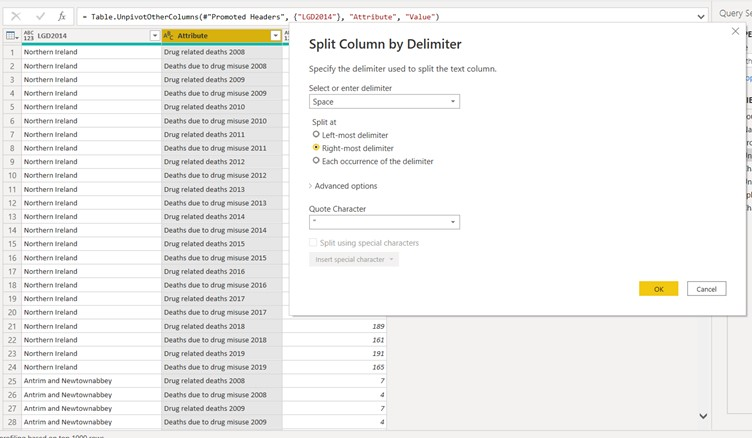
\includegraphics{bi4.jpg}
\caption{Splitting by Delimiters.}
\end{figure}

We want to split this column into two new columns using a delimiter. The best one to choose here is the Space delimiter. We want to split at the \textbf{right-most} delimiter as there is a space right before each year but none after the year. Select these settings and click OK. Change the titles of the columns by \textbf{double clicking} the \textbf{column header}. Finalize your changes by clicking on the \textbf{Home ribbon} and \textbf{Close \& Apply}. As soon as you click Close \& Apply in the Power Query Editor the Power Query Editor will close and the Power BI Desktop Report View will be visible.

These are two of the most common data transformations that data sets will need to have applied to them.

\hypertarget{visualising-data}{%
\section{Visualising Data}\label{visualising-data}}

Power BI is commonly associated with the ability to create impactful, interactive data visualizations. Before we start making visuals it's worth detailing some of the panes and views available to us:

\begin{figure}
\centering
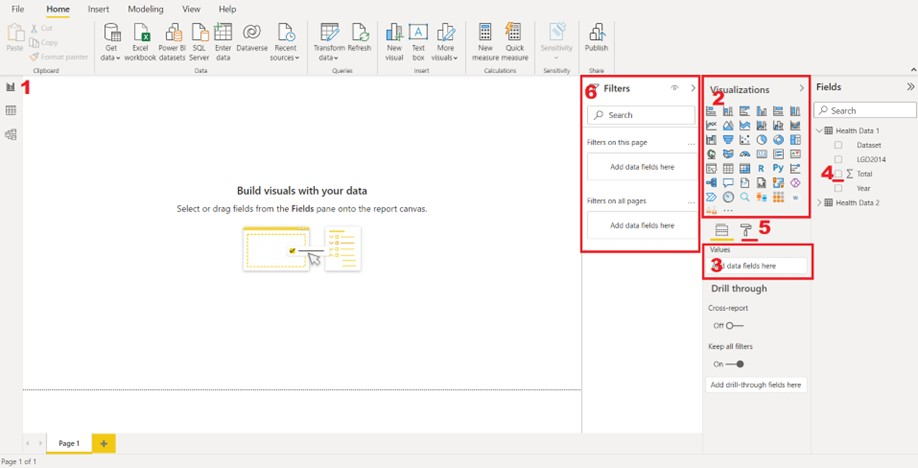
\includegraphics{bi5.jpg}
\caption{Navigating the user interface.}
\end{figure}

\begin{enumerate}
\def\labelenumi{\arabic{enumi}.}
\item
  \textbf{The Report View}: This is the button that will open up the Report canvas and allow us to create visuals using the visuals area. Below the report view button are two more buttons. These provide access to the \textbf{data view} and the \textbf{model view}.
\item
  \textbf{Visuals Area}: This is where we can choose which visual we would like to use. Each of the icons represents a type of visualization. Clicking these icons will generate a visual that we can start to work with. Once custom visuals are added they will appear here as well.
\item
  \textbf{Field Area}: This area will change depending on the visual but it is where we place the variables (Total, Year\ldots{} etc.) that we will use within the selected visual.
\item
  \textbf{Field Pane}: This pane contains the fields we have to choose from to add to our visual. Initially this is populated by the variables contained in data sources but it is possible to add new variables or measures through the Power Query Editor.
\item
  \textbf{Format Area}: This is where we can decide on the formatting of our visuals. You can customise colours or make changes to axes add borders and change font sizes\ldots{} etc.
\item
  \textbf{Filters Area}: This is where we can apply filters of various scopes. We can apply page-level filters which will affect all the visuals on the selected page. We can apply Report-level filters which will affect every visual in the entire Power BI Report and we can apply Visual-level filters which will be applied only to specific visualizations.
\end{enumerate}

\hypertarget{creating-a-line-chart}{%
\subsection{Creating a Line-Chart}\label{creating-a-line-chart}}

We're going to create a \textbf{line-chart visual} that shows both drug related deaths and deaths due to drug misuse. We want to show the totals for each over time and we want to be able to filter by local government district.

The first step in creating any visual is to go to the \textbf{Visualizations pane} on the right-hand side of the UI. Here you can see a range of different visualization icons representing their respective chart. Along the top row are bar charts, in the second row are line charts, area charts and a ribbon chart, below these are pie charts, maps, cards, and even tools to create custom Python and R visuals (Plotly, Matplotlib and Seaborn are three commonly used Python plotting libraries). Find the Icon for the \textbf{Line Chart} and click it. A new visual object will appear on the canvas with a prompt to select or drag fields to populate this visual.

Drag the \textbf{``Year'' field} from the \textbf{fields pane} into the \textbf{Axis box} in the field area. Drag the \textbf{``Total'' field} into the \textbf{Values box}.

You should get a line-chart that looks like this:

\begin{figure}
\centering
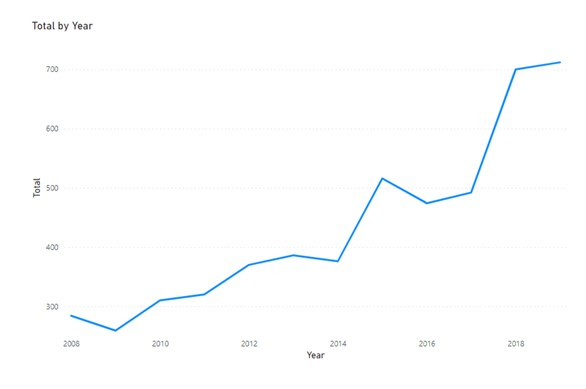
\includegraphics{bi6.jpg}
\caption{The first line chart.}
\end{figure}

There is something not quite right about this visual. We plotted Total by Year but what is it a total of? Our data contained totals for each Local Government District and for two different data sets. Currently, the data for each year is being summed. We are looking at a line chart showing the sum of all Local Government District drug related deaths and deaths due to drug misuse. We can tell this is the case at a glance by looking to the \textbf{Fields Pane} where the \textbf{Total} has a summation sign (\(\sum\)) to the left of it.

Drag the \textbf{Dataset field} into the \textbf{Legend box} to separate out the data sets. You should see a line-chart like this:

\begin{figure}
\centering
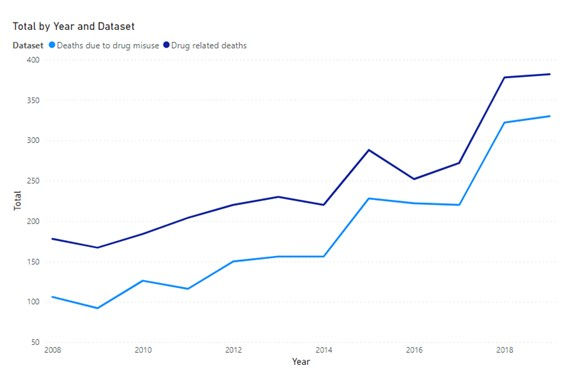
\includegraphics{bi7.jpg}
\caption{Line chart.}
\end{figure}

This is closer to what we had hoped to show but it's still summing over the local government districts. This is where the \textbf{Slicer visualization} becomes useful. Although, we don't need to use slicers, we could also use the filters pane to simply remove the districts we don't want to be summed. This can be useful when datasets contain rows of data that we aren't interested in.

\hypertarget{the-slicer-visual}{%
\subsection{The Slicer Visual}\label{the-slicer-visual}}

The \textbf{Slicer visual} is used when we want our users to be able to filter by something that isn't used inside our visuals. The slicer visual only allows one field to be assigned to it. Passing text data into the field will generate a list of check boxes which can be ticked or unticked. Passing numeric data into the field will generate a slider which can be moved from one numeric value to the next (useful for dates).

Before we create a new Slicer visual it is important to make sure we have deselected the line-chart visual otherwise clicking on a new visual icon will convert this visual into the selected visual type. We don't want to convert our visual, we want an entirely new visual. \textbf{Click} on \textbf{the canvas} behind the line-chart visual then in the \textbf{visualizations pane} locate the \textbf{Slicer visual} and click on it. A new visual object will appear. Drag \textbf{LGD2014} from the \textbf{Fields Pane} into the \textbf{Field box} in the Field Area. A checkbox list of local government districts should populate in the visual object on the canvas. It should look like this:

\begin{figure}
\centering
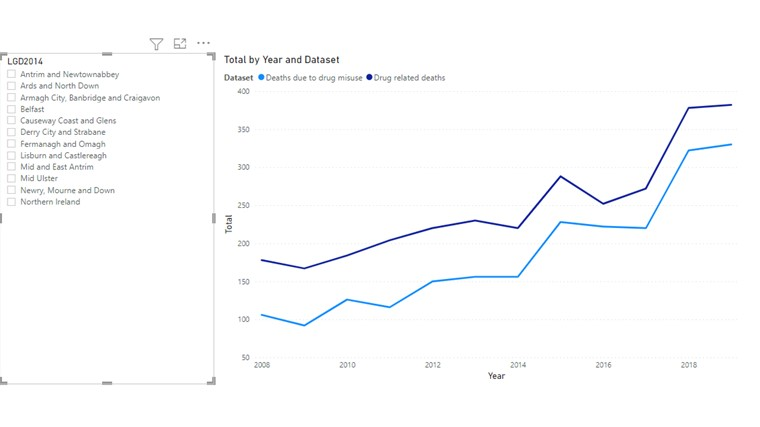
\includegraphics{bi8.jpg}
\caption{Filtering data by local government district (LGD).}
\end{figure}

\hypertarget{the-format-area}{%
\subsection{The Format Area}\label{the-format-area}}

We now have a line-chart that shows both deaths due to drug misuse and drug related deaths but if we control click multiple local government districts it sums them together. We can change this behaviour by formatting the slicer visual.

Click the \textbf{slicer visual} then click on the \textbf{Format area selector} (the icon that looks like a paint roller). We will be presented with a list of different attributes that we can change. We can change the title, the background, the border and we can add shadows. The important attribute we want to change however is \textbf{Selection controls}. Click the \textbf{drop-down arrow} beside \textbf{Selection controls} and toggle \textbf{single select} on. The result should be something that looks like this:

\begin{figure}
\centering
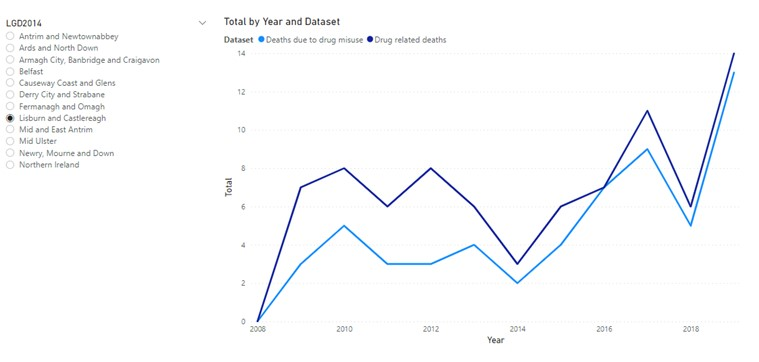
\includegraphics{bi9.jpg}
\caption{Filtering data by local government district (LGD) and selecting different regions.}
\end{figure}

This presentation style has positives and negatives. It's useful if we know we have lots of visitors who only want to know about their local government district but it's not very good for comparing different districts. We're going to use what we have done so far to build a new visual that allows users to directly compare their local government district to another.

Our line-chart visual will use LGD2014 as its legend. Our slicer will have to enable multiple selection. We may also want to include additional slicers to filter the visual by year and by the data set we would like to compare. We will also convert the visual type to a stacked bar chart. The final result should look like this:

\begin{figure}
\centering
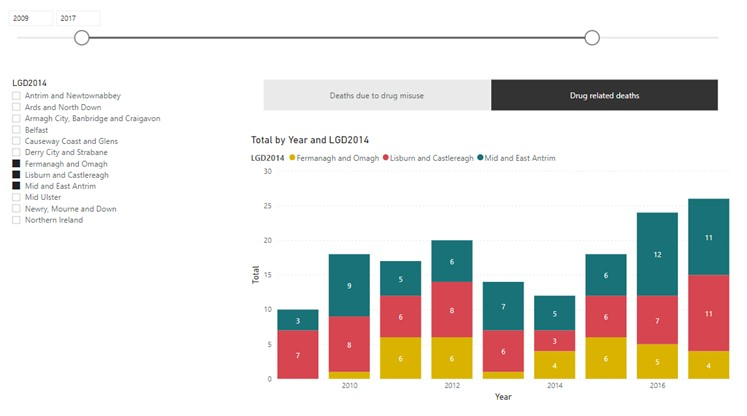
\includegraphics{bi10.jpg}
\caption{The Finished Product.}
\end{figure}

The new visual should allow us to check multiple boxes and add to the stacked bar chart. We should also be able to filter by year using the slider at the top and we should be able to select the data set we're interested in using the buttons above the visual.

\hypertarget{adding-a-new-page}{%
\section{Adding a New Page}\label{adding-a-new-page}}

We can add a new page to our report by clicking the plus sign \textbf{+} next to the \textbf{Page 1 tab} at the bottom of the canvas. It makes sense however to duplicate our existing page since we can re-use some of our existing work. \textbf{Right click} on the \textbf{Page 1 tab} and select \textbf{Duplicate Page}.

Select the \textbf{line-chart visual} and change the \textbf{legend} in the \textbf{Fields Area} from \textbf{Dataset} to \textbf{LGD2014} by clicking on the \textbf{X} to the right of \textbf{Dataset} and dragging in \textbf{LGD2014} from the \textbf{Fields Pane}. Now click on the \textbf{stacked column char}t icon in the \textbf{Visualizations Pane} to convert the visual. Some conversions work better than others, it's always worth checking that the visual is showing the same data before and after conversion. A conversion from a stacked bar chart to a card visual or KPI visual may not be the best choice for instance.

We will need to edit the location filter (the slicer) to allow for multiple selections. Click on the \textbf{slicer visual} and go to the \textbf{Format Area}. Under \textbf{Selection Controls} toggle \textbf{Single Select} to \textbf{off} and ensure that \textbf{Multi-select with CTRL} is toggled to the \textbf{on} position and \textbf{Show ``Select All'' Option} is toggled to the \textbf{off} position. We can now select multiple local government districts and they should stack on top of one another in the stacked bar chart visual. We will need two new slicer visuals.

Click on the canvas to ensure no visuals are selected. Select the \textbf{Slicer Visual} in the visualizations pane. Drag the \textbf{Year field} into the \textbf{Field box}. The slicer should automatically detect numeric data and generate a slider that takes values in the range 2008 to 2019.

We need one more slicer. Again ensure no visuals are currently selected and select the \textbf{Slicer Visual}. Drag the \textbf{Dataset} field into the slicer's field. A checkbox will be generated. We would prefer buttons this time, so go to the \textbf{Format Area} and select the \textbf{General} option. Scroll down until you see \textbf{Orientation}. Click on the drop down menu and select \textbf{Horizontal}. Under \textbf{Selection Controls} you might want to toggle \textbf{Single select} to \textbf{on}.

Finally, we can add some data labels to our visual. Select the line-chart visual by clicking on it. In the Format Area scroll down until you see \textbf{Data Labels} and toggle them \textbf{on}.

\hypertarget{navigation}{%
\section{Navigation}\label{navigation}}

\hypertarget{arrows}{%
\subsection{Arrows}\label{arrows}}

Up to this point we have mostly made use of the Home ribbon but there are other important ribbons when designing reports. The \textbf{Insert ribbon} for instance allows us to insert elements into our report that aren't necessarily data visualizations. We can insert text boxes, buttons, shapes and images. These are all useful for providing additional information on visualizations, explaining data or navigation. We're going to create navigation buttons.

Add two new pages to your report using the plus icon next to the page tabs at the bottom of the canvas. Click onto the first of those pages. Then navigate to the \textbf{Insert ribbon} and click on \textbf{Buttons} then on the \textbf{right arrow}.

\begin{figure}
\centering
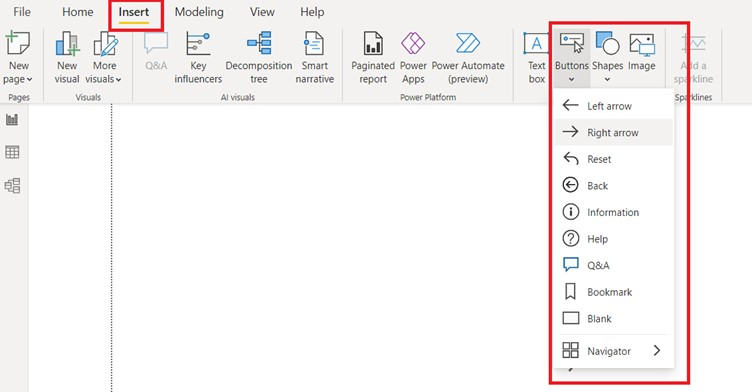
\includegraphics{bi11.jpg}
\caption{Inserting arrows.}
\end{figure}

Repeat this process on the second page but this time select the \textbf{Left arrow}. If the Left arrow is selected you will see the visualisations pane disappear and the entire pane will be taken up by the format pane. Scroll down until you find \textbf{Action}. Toggle \textbf{Action} to \textbf{on} and select \textbf{Page navigation} in the \textbf{Type menu} and \textbf{Page 1} (or whatever page you want this arrow to direct to) in the \textbf{Destination menu}.

\begin{figure}
\centering
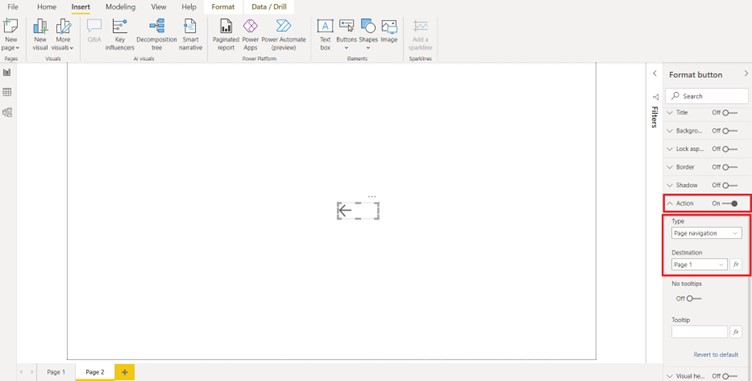
\includegraphics{bi12.jpg}
\caption{Left Arrow Navigation.}
\end{figure}

If you \textbf{CTRL+Click} on the \textbf{Left arrow} it should now take you to \textbf{Page 1}. When your Power BI Report is published users won't need to CTRL+Click it will just happen with a click. We can repeat these steps for the Right Arrow on Page 1 to cycle between the pages.

\hypertarget{buttons}{%
\subsection{Buttons}\label{buttons}}

Another useful element that we can insert is the \textbf{Button}. The Button can serve just about any purpose. It can be filled with color and used as a banner or a footer; it can be used as a navigation tool thanks to the actions we just used; and it can be used as a display behind a visual.

Create a new page. Find \textbf{Buttons} on the \textbf{Insert ribbon}. Click it and select \textbf{Blank}. An outlined box should appear. You can click the edges of this to resize it. Try to take up the whole width available and just less than 20\% of the height. It doesn't need to be exact, just resize to whatever looks natural as a header for a title.
Click on the resized button when you're finished. In the \textbf{Format Button pane} toggle \textbf{Outline} to \textbf{off} and toggle \textbf{Icon} to \textbf{off}. Toggle \textbf{Fill} to \textbf{on} and expand the fill menu and select a new color for your header. Change the transparency settings if you like. Next, find the \textbf{Text toggle} and toggle it \textbf{on} if it isn't already. Open the \textbf{Text menu} by clicking the drop-down arrow. In the text box type a title for your new page. You can change the font color and text size and the font below the text entry box.

Add another button but this time resize it to whatever size you think appropriate for a navigation button. Repeat the steps above to add colour and text to the button. Then you can use the action menu, like we did when we created the left and right arrows, to give the button navigation properties.

With any luck you should be able to replicate the kind of user interface you see in a \textbf{single page web app} or a \textbf{mobile app}.

\begin{figure}
\centering
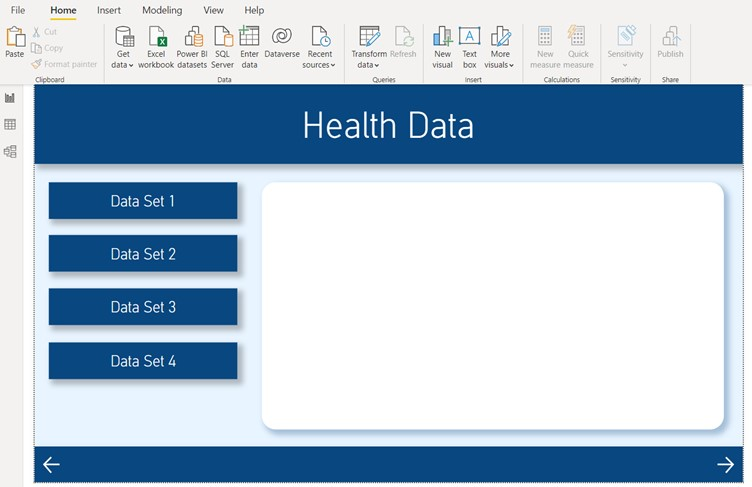
\includegraphics{bi13.jpg}
\caption{Buttons used to create links between pages.}
\end{figure}

\hypertarget{indexing}{%
\section{Indexing}\label{indexing}}

This example will show you how to create a bar chart visual of sales by month. This sounds simple but often when trying to visualise data categorised by month the bars for each month are sorted by alphabetical order rather than the order in which the months occur.

Start a new project and click \textbf{Enter Data}.

Enter the months of the year in the available column and change the column title to ``Month''.

Press the \textbf{+} Icon at the top right to create a new column, title it ``Sales'' and enter some dummy sales data.

\begin{figure}
\centering
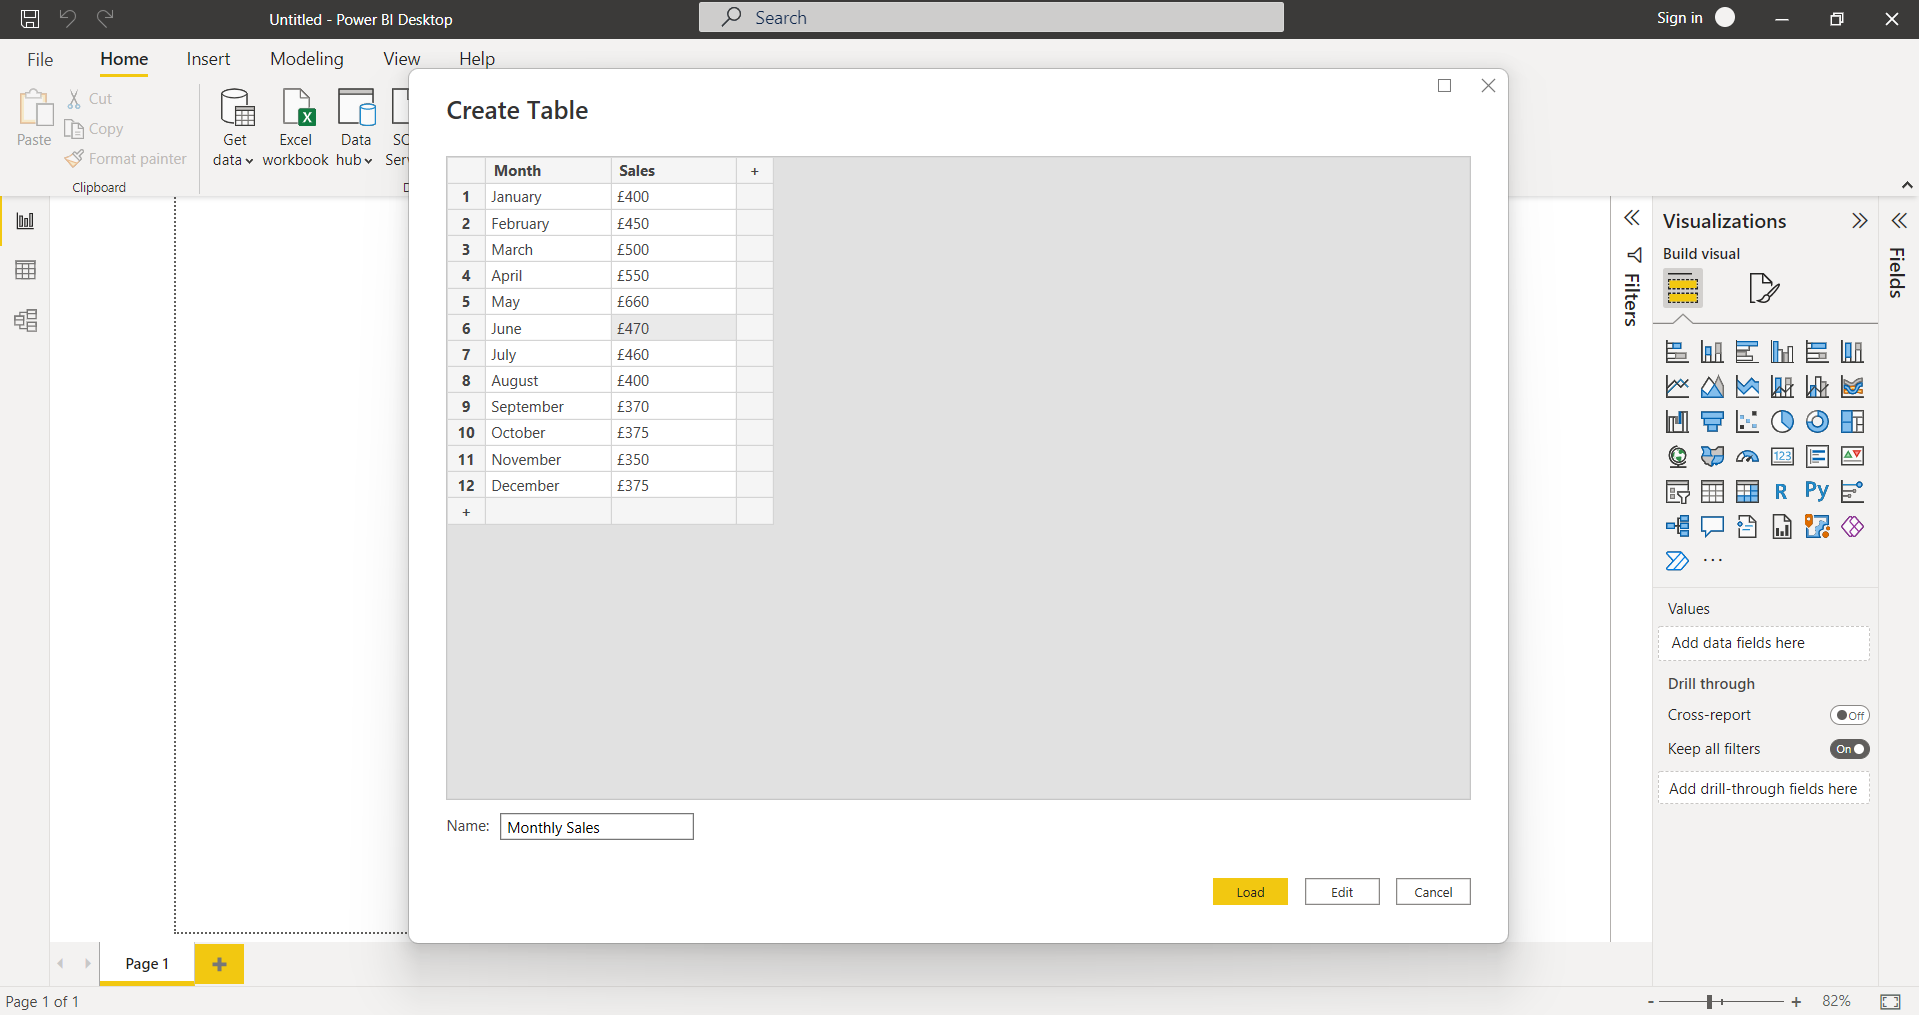
\includegraphics{bi14.png}
\caption{Entering data}
\end{figure}

Load the data.

Create a bar chart visualisation with ``Month'' in the X-axis field and ``Sales'' in the Y-axis field.

Once the visualisation has been created click the \textbf{\ldots{}} icon for more options and sort the axis by month. The x-axis will be sorted by month but it will be sorted alphabetically.

To rectify this we need to create an \textbf{index}.

Click on \textbf{Transform Data} and navigate to ``Monthly Sales''. In \textbf{Applied Steps} pane on the right hand side there will be a step called \textbf{Source} with a cog icon to the right of it. Click on the cog. This will open up the editor you used to input the data. Create a new column by clicking the \textbf{+} icon. Call this new column ``Index'' and write the number 1 in the first empty row. Write the number 2 in the next row and the number 3 in the next. Continue until each Month has a corresponding numerical index.

\begin{figure}
\centering
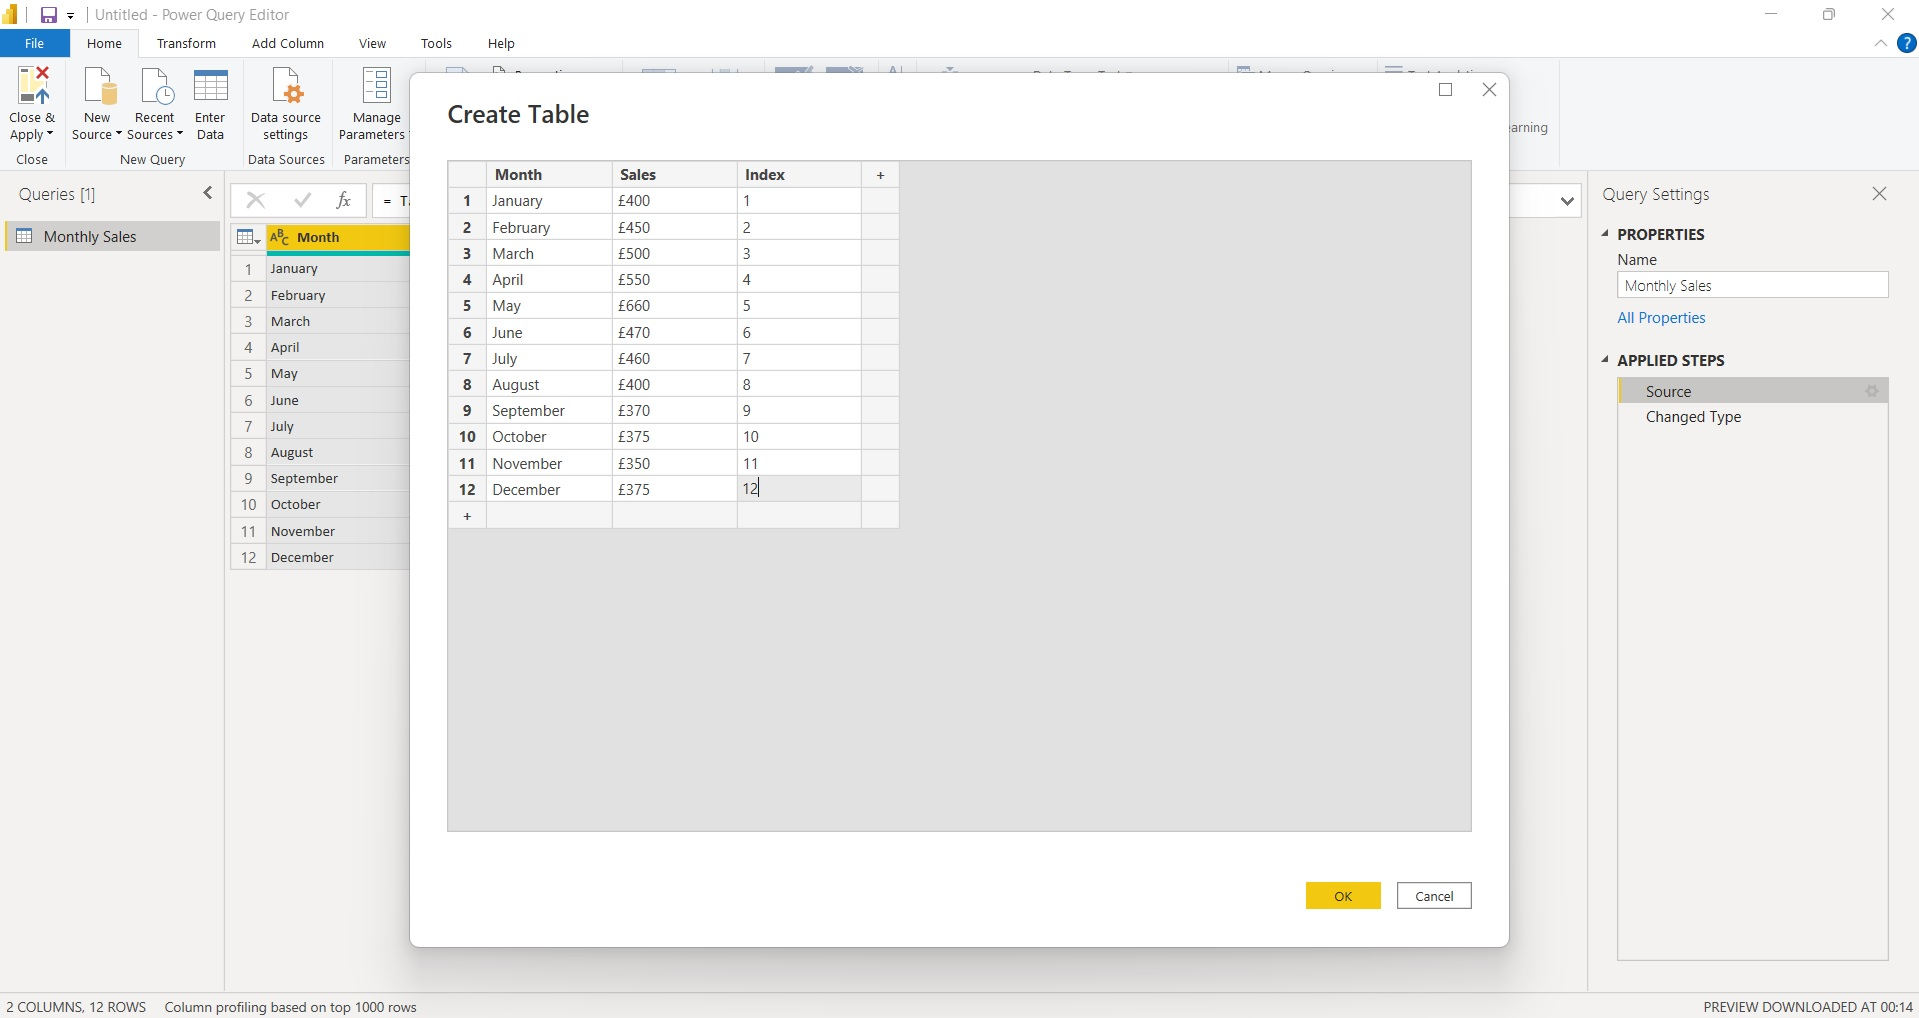
\includegraphics{bi15.jpg}
\caption{Creating an index}
\end{figure}

When finished, click \textbf{OK} then \textbf{Close \& Apply}.

Go to the data view, click on the ``Month'' column and find the \textbf{Sort by column} option in the \textbf{column tools} ribbon and select ``Index''.

\begin{figure}
\centering
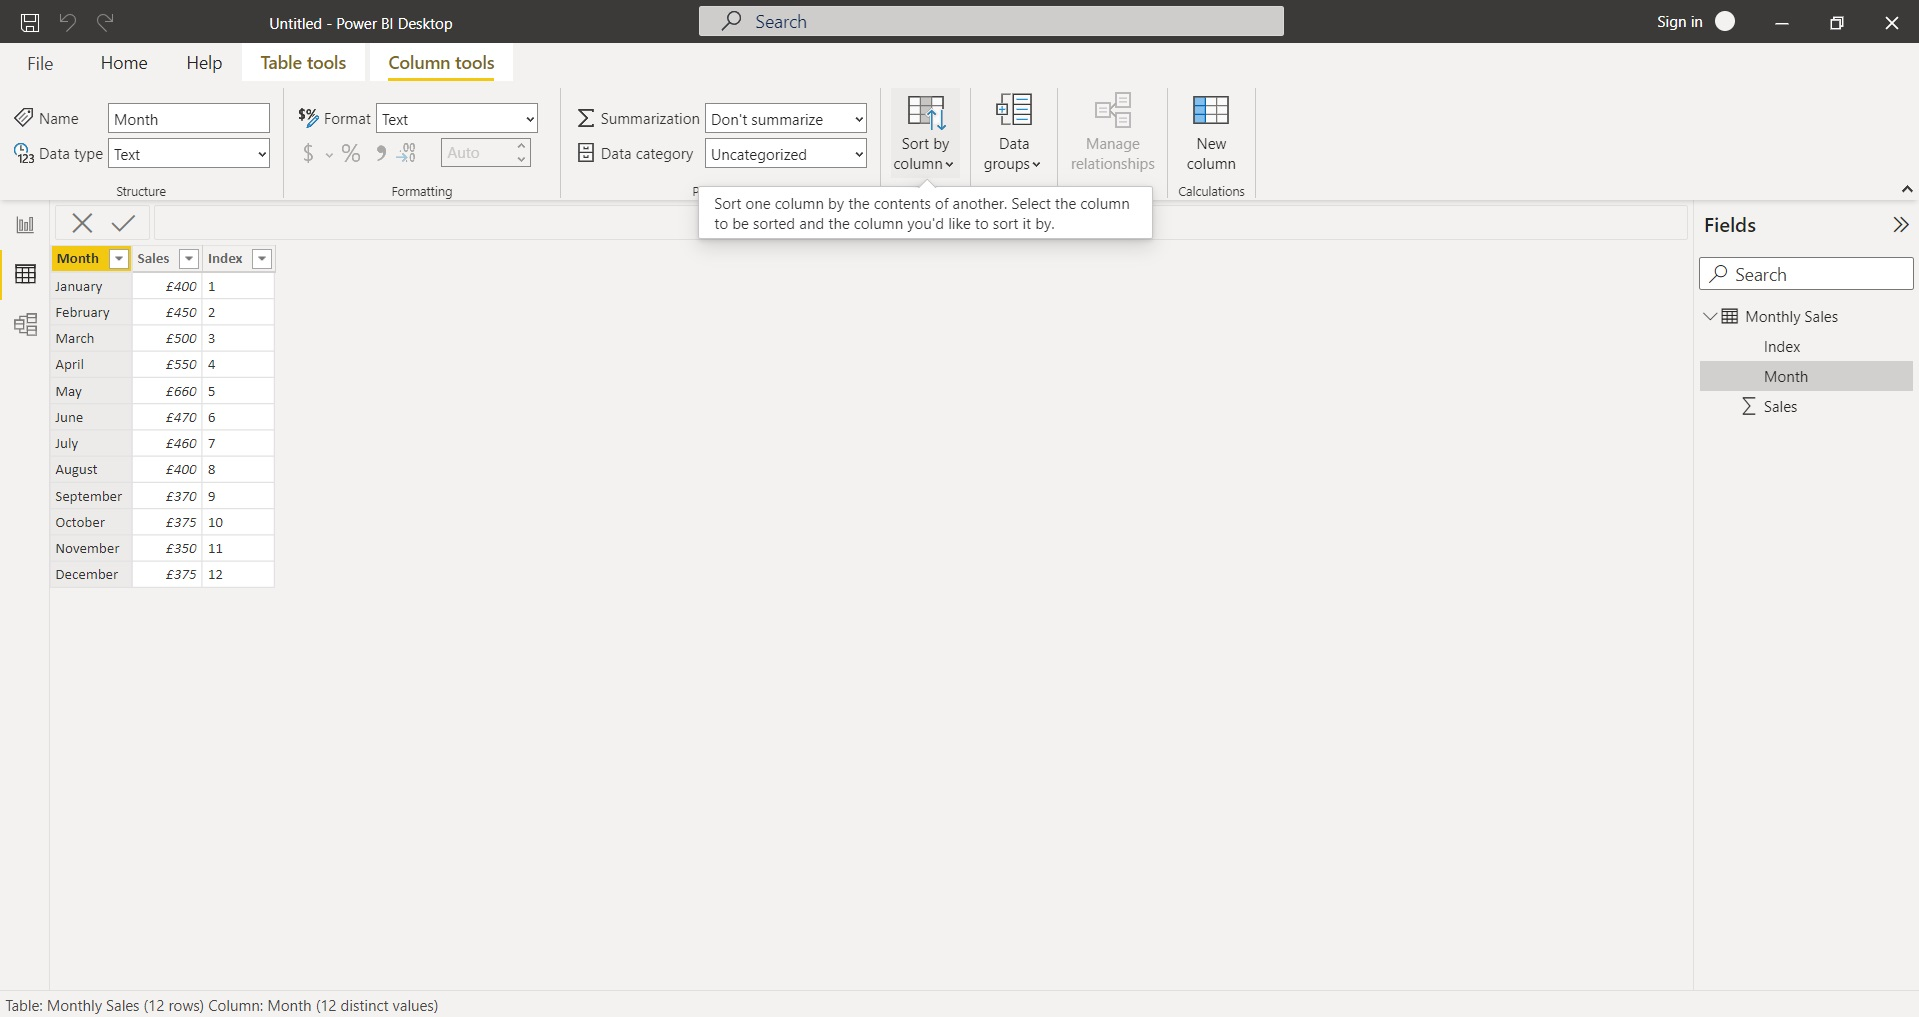
\includegraphics{bi16.jpg}
\caption{Sorting by column}
\end{figure}

Return to the visualisation and the months should now be sorted in the correct order.

\hypertarget{relationships}{%
\section{Relationships}\label{relationships}}

\hypertarget{publishing}{%
\section{Publishing}\label{publishing}}

\hypertarget{additional-resources}{%
\section{Additional Resources}\label{additional-resources}}

This content has been designed to provide a tour of the main features of Power BI reports. It has skipped a lot of detail to try and give a broad overview of what is possible with Power BI and provide the basic skills needed to start experimenting with the software package. The \href{https://docs.microsoft.com/en-us/power-bi/fundamentals/}{Power BI Documentation} should provide a more in depth look at the fundamentals. Microsoft Learn has a number of \href{https://docs.microsoft.com/en-us/learn/modules/get-started-with-power-bi/}{modules} dedicated to Power BI which are mostly related to Data Analysis learning pathways. Completing these modules will be useful for consolidating the fundamentals and learning more about Power BI in greater detail. If you're really interested then it might be worth reading into \href{https://docs.microsoft.com/en-us/dax/}{Data Analysis Expressions (DAX)} which is a library of functions that can be used to build formulas and expressions in Power BI, Analysis Services, and Power Pivot in Excel data models. This is especially useful in Power Query Editor.

\hypertarget{python}{%
\chapter{Python}\label{python}}

\hypertarget{introduction-1}{%
\section{Introduction}\label{introduction-1}}

\hypertarget{variables}{%
\subsection{Variables}\label{variables}}

In programs, information can be stored in variables. Variables are labels to help with storing and retrieving information from memory. There are different types of variables, which include:

\begin{itemize}
\item
  \textbf{Integers} - positive and negative integers up to a high limit, for instance, \(-2, -1, 0, 1, 2\). A variable can be declared as an integer - or converted to one - using the int() function.
\item
  \textbf{Floating point numbers} - Positive and negative whole numbers with a decimal point. For instance \(0.1, 2.5, 50.294, -75.943\). A variable can be declared as a floating point number - or converted to one - using the float() function.
\item
  \textbf{Strings} - strings are arrays of bytes representing unicode characters. A variable can be declared as a string using quotation marks or the str() function which can also be used to convert a variable to a string type.
\item
  \textbf{Boolean} - booleans represent one of two values, either True or False. In programming you frequently need to know if an expression is true or false and booleans are typically useful for this. A variable can be declared boolean - or converted to one - using the bool() function
\item
  \textbf{Complex numbers} - Numbers that satisfy \(i^2=-1\), written as \(a+bi\) where \(a\) and \(b\) are real numbers. These are rarely, if ever, encountered in research however they can be useful when optimising advanced scripts.
\end{itemize}

We declare variables by giving them a name and setting them equal to some value. Variables can be printed to screen using the print() function and the type() function can be used to probe a variable and discover what type of variable it is.

Variables are declared by writing a variable name and using the equals sign to indicate the value to be associated with that name. Alternatively, functions like int() or float() can be used although they are not typically needed as Python is able to interpret the type without being explicitly told using these functions.

\begin{Shaded}
\begin{Highlighting}[]
\CommentTok{\# Below are some examples of variable declaration.}

\NormalTok{intVar}\OperatorTok{=}\DecValTok{1}
\NormalTok{floatVar}\OperatorTok{=}\FloatTok{2.13}
\NormalTok{stringVar}\OperatorTok{=}\StringTok{"This is a string"}
\NormalTok{boolVar}\OperatorTok{=}\VariableTok{True}
\NormalTok{compVar}\OperatorTok{=}\BuiltInTok{complex}\NormalTok{(}\DecValTok{3}\NormalTok{,}\DecValTok{2}\NormalTok{)}

\CommentTok{\#Variables can be printed to the screen using the print() function. }

\BuiltInTok{print}\NormalTok{(intVar, floatVar, stringVar, boolVar, compVar)}
\end{Highlighting}
\end{Shaded}

\begin{verbatim}
## 1 2.13 This is a string True (3+2j)
\end{verbatim}

Using the \textbf{type()} function with the variable name as an argument will return the type of the variable. In this example the type() function is applied to the intVar variable. and the \textbf{print()} function is used to print the result to the screen. These functions could be applied one at a time but it's also possible to place a function within a function. The innermost function is performed first.

\begin{Shaded}
\begin{Highlighting}[]
\CommentTok{\# Functions can be called inside other functions.}

\BuiltInTok{print}\NormalTok{(}\BuiltInTok{type}\NormalTok{(intVar))}
\end{Highlighting}
\end{Shaded}

\begin{verbatim}
## <class 'int'>
\end{verbatim}

Boolean values refer to logic and can be useful for testing. For instance, given two variables we can use \textbf{operators} to test whether one is greater than, less than or equal to the other. The result of this test will be a boolean.

\begin{Shaded}
\begin{Highlighting}[]
\NormalTok{i }\OperatorTok{=} \DecValTok{20}
\NormalTok{j }\OperatorTok{=} \DecValTok{30}

\BuiltInTok{print}\NormalTok{(i }\OperatorTok{\textless{}}\NormalTok{ j)}
\end{Highlighting}
\end{Shaded}

\begin{verbatim}
## True
\end{verbatim}

\hypertarget{examples}{%
\subsubsection{Examples}\label{examples}}

\begin{enumerate}
\def\labelenumi{\arabic{enumi}.}
\tightlist
\item
  Print the words ``Hello world'' to the screen.
\end{enumerate}

\begin{Shaded}
\begin{Highlighting}[]
\CommentTok{\# Use the print() function.}

\BuiltInTok{print}\NormalTok{(}\StringTok{"Hello world"}\NormalTok{)}
\end{Highlighting}
\end{Shaded}

\begin{verbatim}
## Hello world
\end{verbatim}

\begin{enumerate}
\def\labelenumi{\arabic{enumi}.}
\setcounter{enumi}{1}
\tightlist
\item
  Assign two integer values to the variables named firstVar and secondVar. Assign any values you like. Print the values to the screen.
\end{enumerate}

\begin{Shaded}
\begin{Highlighting}[]
\CommentTok{\# Assign values to variable names with the \textquotesingle{}equals\textquotesingle{} operator \textquotesingle{}=\textquotesingle{}.}

\NormalTok{firstVar }\OperatorTok{=} \DecValTok{20}
\NormalTok{secondVar }\OperatorTok{=} \DecValTok{40}

\BuiltInTok{print}\NormalTok{(firstVar, secondVar)}
\end{Highlighting}
\end{Shaded}

\begin{verbatim}
## 20 40
\end{verbatim}

\begin{enumerate}
\def\labelenumi{\arabic{enumi}.}
\setcounter{enumi}{2}
\tightlist
\item
  Write a program that calculates the average of the following set of numbers:
\end{enumerate}

\[ 2,3,4,5,20.\]

\begin{Shaded}
\begin{Highlighting}[]
\CommentTok{\# Assign the values to variables.}

\NormalTok{firstVar }\OperatorTok{=} \DecValTok{2}
\NormalTok{secondVar }\OperatorTok{=} \DecValTok{3}
\NormalTok{thirdVar }\OperatorTok{=} \DecValTok{4}
\NormalTok{fourthVar }\OperatorTok{=} \DecValTok{5}
\NormalTok{fifthVar }\OperatorTok{=} \DecValTok{20}

\CommentTok{\# The following line of code can be used to find the average:}

\NormalTok{average }\OperatorTok{=}\NormalTok{ (firstVar }\OperatorTok{+}\NormalTok{ secondVar }\OperatorTok{+}\NormalTok{ thirdVar }\OperatorTok{+}\NormalTok{ fourthVar }\OperatorTok{+}\NormalTok{ fifthVar)}\OperatorTok{/}\DecValTok{5}

\BuiltInTok{print}\NormalTok{(average)}
\end{Highlighting}
\end{Shaded}

\begin{verbatim}
## 6.8
\end{verbatim}

\hypertarget{mathematical-operations}{%
\subsection{Mathematical Operations}\label{mathematical-operations}}

Note that in Python we can add, subtract, multiple and divide in equations with the symbols \(+, -, *, /.\) and brackets can be used to ensure the result of the calculations inside the brackets are calculated with highest priority. The table below outlines the various mathematical operations that can be performed.

\begin{longtable}[]{@{}
  >{\raggedleft\arraybackslash}p{(\columnwidth - 4\tabcolsep) * \real{0.3548}}
  >{\raggedleft\arraybackslash}p{(\columnwidth - 4\tabcolsep) * \real{0.3548}}
  >{\raggedleft\arraybackslash}p{(\columnwidth - 4\tabcolsep) * \real{0.2903}}@{}}
\caption{\label{tab:table13}Basic Mathematical Operations}\tabularnewline
\toprule
\begin{minipage}[b]{\linewidth}\raggedleft
Operation
\end{minipage} & \begin{minipage}[b]{\linewidth}\raggedleft
Example
\end{minipage} & \begin{minipage}[b]{\linewidth}\raggedleft
Description
\end{minipage} \\
\midrule
\endfirsthead
\toprule
\begin{minipage}[b]{\linewidth}\raggedleft
Operation
\end{minipage} & \begin{minipage}[b]{\linewidth}\raggedleft
Example
\end{minipage} & \begin{minipage}[b]{\linewidth}\raggedleft
Description
\end{minipage} \\
\midrule
\endhead
+ & a=b+c & a takes the value of b+c \\
+= & a+=b & a takes the value of a+b \\
- & a=b-c & a takes the value of b-c \\
-= & a-=b & a takes the value of a+b \\
* & a=b*c & a takes the value of b*c \\
*= & a*=b & a takes the value of a*b \\
/ & a=b/c & a takes the value of b/c \\
/= & a/=b & a takes the value of a/b \\
** & a=b**c & a takes the value of b to the power c \\
**= & a**=b & a takes the value of a to the power b \\
// & a=b//c & a takes the value of floor division of b by c \\
//= & a//=b & a takes the value of floor division of a by b \\
\% & a=b\%c & a takes the value of b modulo c \\
\%= & a\%=b & a takes the value of a modulo b \\
\bottomrule
\end{longtable}

\hypertarget{functions}{%
\subsection{Functions}\label{functions}}

A \textbf{function} is a group of related statements forming reusable code that is used to perform some specific task. The task can be anything: a simple calculation or a complex iterative process or even a series steps in an algorithm.

Functions make writing code easier since often we might want to repeat the same piece of code several times, instead of rewriting or copying and pasting that same chunk of code we can write a function once and call it each time it is needed.

Python has some `in-built' functions but we can create our own custom functions too.

\hypertarget{in-built-functions}{%
\subsubsection{In-built Functions}\label{in-built-functions}}

We have already encountered several in-built functions: int(), float(), bool(), str(), complex(), type() and print().

Some other useful in-built functions are:

len() - the \textbf{len()} function can be used to tell us how long a particular variable or object is.

\begin{Shaded}
\begin{Highlighting}[]
\NormalTok{a }\OperatorTok{=} \StringTok{"Hello World!"}

\NormalTok{b }\OperatorTok{=} \BuiltInTok{len}\NormalTok{(a)}

\BuiltInTok{print}\NormalTok{(b)}
\end{Highlighting}
\end{Shaded}

\begin{verbatim}
## 12
\end{verbatim}

help() - the \textbf{help()} function can return useful help on functions, variables and objects.

\begin{Shaded}
\begin{Highlighting}[]

\BuiltInTok{help}\NormalTok{(}\BuiltInTok{len}\NormalTok{)}
\end{Highlighting}
\end{Shaded}

\begin{verbatim}
## Help on built-in function len in module builtins:
## 
## len(obj, /)
##     Return the number of items in a container.
\end{verbatim}

input() - the \textbf{input()} function can be used to accept user inputs when assigning values to variables.

\hypertarget{custom-functions}{%
\subsubsection{Custom Functions}\label{custom-functions}}

\hypertarget{data-structures}{%
\subsection{Data Structures}\label{data-structures}}

\hypertarget{exceptions-try-and-except}{%
\subsection{Exceptions, Try and Except}\label{exceptions-try-and-except}}

\hypertarget{loops-and-iterating}{%
\subsection{Loops and Iterating}\label{loops-and-iterating}}

\hypertarget{built-in-functions}{%
\subsection{Built in Functions}\label{built-in-functions}}

\hypertarget{managing-data}{%
\section{Managing Data}\label{managing-data}}

\hypertarget{dataframes}{%
\subsection{Dataframes}\label{dataframes}}

\hypertarget{visualisations}{%
\section{Visualisations}\label{visualisations}}

\hypertarget{matplotlib}{%
\subsection{Matplotlib}\label{matplotlib}}

\hypertarget{seaborn}{%
\subsection{Seaborn}\label{seaborn}}

\hypertarget{bokeh}{%
\subsection{Bokeh}\label{bokeh}}

\hypertarget{using-python}{%
\section{Using Python}\label{using-python}}

\hypertarget{apis}{%
\subsection{APIs}\label{apis}}

\hypertarget{web-scraping}{%
\subsection{Web Scraping}\label{web-scraping}}

\hypertarget{automation}{%
\subsection{Automation}\label{automation}}

\hypertarget{r}{%
\chapter{R}\label{r}}

  \bibliography{book.bib,packages.bib}

\end{document}
